%======================================================================
%   Zak Webb
%   Ph. D. Thesis
%   Department of Physics and Astronomy
%   University of Waterloo
% 
%   Scattering on Graphs
%======================================================================


\documentclass[../thesis-main/thesis-main]{subfiles}
\begin{document}

\chapter{Scattering on graphs}

Graph scattering has been an illuminating example of the uses of quantum algorithms.  The original motivation for quantum walks (the quantum generalization to classical random walks), these scattering ideas make use of scattering problems in the continuum to give intuition on problems related to quantum mechanics.

\todo{Give a much better introduction to this idea of graph scattering, with references}


\section{Free particles in the continuum}

Let us first take a look at one of the most simple quantum systems seen in any quantum mechanics text (e.g., \cite{GriQM} or \cite{SakMQM}): a free particle in one dimension.  Without any potential or interactions, we have that the time independent Schr\"{o}dinger equation reads
\begin{equation}
  \frac{\partial^2}{\partial x^2} \psi(x) = -\frac{2m}{\hbar^2}E \psi(x) = -k^2 \psi(x),
\end{equation}
which requires the (unnormalizable) solutions,
\begin{equation}
  \psi(x) = A \exp(- i k x) + B \exp(i k x) \label{eq:simple_motivating_momentum_states}
\end{equation}
for real $k$ and for arbitrary constant $A$ and $B$.  These \textit{momentum states} correspond to particles travelling with momentum $k$ along the real line, and form a basis for the entire Hilbert space.

While these momentum states are useful for understanding the propagation of particles in the quantum setting, if we want to understand more complicated behavior we need to change the potential energy of the system.  In particular, we will now include some finite-range potential $V$ that is non-zero only for $|x| < d$ for some constant $d$, so that outside this range the eigenstates remain unchanged.  The only difference is that we will deal with a superposition of states for each energy instead of the pure momentum states, forcing some relation between the $A$ and $B$ of equation \eq{simple_motivating_momentum_states}.  Namely, the eigenstates of this system become
\begin{equation}
  \psi(x) = \begin{cases}
    \exp(-i k x) + R(k) \exp(i k x) & x \leq -d\\
    T(k) \exp(- i k x) & x \geq d\\
    \phi(x,k) & |x| \leq d
    \end{cases}
\end{equation}
for some functions $R(k)$, $T(k)$, and $\phi(x,k)$ that depends on the interaction $V$.  As intuition, these states can be seen as a particle with momentum $k$ coming in from the left, hitting the potential, and then scattering (which motivates the $T$ and $R$ labels).  

In addition to these scattering states, it is also possible for bound states to exist.  These are normalizable states that have most (or all) of their amplitude near the non-zero potential, so that they do not affect scattering states that originate far from the interaction.  They simply exist as additional states in the Hilbert space.


\todo{possibly include a $\delta$-function potential scattering problem in the thesis}


\subsection{Free particles on an infinite path}

With the simple free-particle example in mind, let us now examine the discretized system.  Namely, instead of allowing arbitrary real positions, let us restrict attention to some regular 1-D lattice, such as the natural numbers.  Further, much as there is a natural linear ordering on the positions in the continuum, and in order for a particle to move between $a$ and $b$ it must travel over all positions between $a$ and $b$, in the discretized system we only allow particles to move between adjacent integers.  Explicitly, the position basis for this discretized Hilbert space will be labeled by $n\in \NN$, with transport only allowed between integers that differ by one.

If we then want to understand how this discretized system works, it will be useful to discretize the entire Schr\"{o}dinger equation.  Along those lines, remember that the second derivative of a function $f$ at $x$ can be written as
\begin{align}
  \frac{d^2}{dx^2} f(x) = \lim_{h\rightarrow 0} \frac{f(x+h) - 2 f(x) - f(x-h)}{h^2}.
\end{align}
Since we were originally working in the continuum, we could let $h$ go to zero without any problems.  In our discretize world, however, there exists some smallest difference in $x$, namely 1.  As such, we have that in our discretized space, the operator corresponding to the second position derivative can be written as
\begin{equation}
  \Delta^2 = \sum_{x=-\infty}^\infty \ket{x} \big(\bra{x-1} - 2 \bra{x} + \bra{x+1}\big) = \sum_{x=-\infty}^\infty \big(\ketbra{x}{x-1} + \ketbra{x}{x+1}\big) - 2 \II.
\label{eq:discrete_second_derivative}
\end{equation}
If we then rescale the energy levels, we have that the identity term in the right hand side of \eq{discrete_second_derivative} can be removed, so that $\Delta^2$ on this discretized one-dimensional system is proportional to the adjacency matrix of an infinite path.  

With this representation of the second derivative operator, we can see that when discretized, the time-independent Schr\"{o}dinger equation for a free particle becomes
\begin{equation}
  \Delta^2 \ket{\psi} = \Big(\sum_{x=-\infty}^\infty \big(\ketbra{x+1}{x} + \ketbra{x-1}{x}\big) - 2 \II\Big) \ket{\psi} = E'_{\psi} \ket{\psi}.
\end{equation}
If we rescale the energy term, and then break the vector equation into its components, we find that
\begin{equation}
  \braket{x+1}{\psi} + \braket{x-1}{\psi} = E_\psi \braket{x}{\psi}
\end{equation}
for all $x\in \ZZ$.  Taking motivation from the continuous case,  we then make the ansatz that $\braket{x}{\psi} = e^{i k x}$ for some $k$, and find
\begin{align}
  \braket{x+1}{\psi} + \braket{x-1}{\psi} = e^{i k } e^{i k x} + e^{-ik} e^{ikx} &= E_\psi e^{ik x} = E_\psi \braket{x}{\psi} &\Rightarrow \\ E_\psi &= e^{ik} + e^{-i k} = 2 \cos(k).
\end{align}
If we then use the fact that $E_\psi$ must be real, and that the amplitudes should not diverge to infinity as $x\rightarrow \pm \infty$, we find that the only possible values of $k$ are between $[-\pi,\pi)$.    Hence, in analogy with the continuous case, the eigenbasis of the Hamiltonian corresponds to momentum states, but where the possible momenta only range over $[-\pi,\pi)$.  We represent this momentum state with momenta $k$ as $\ket{\tilde{k}}$.

Additionally, we can discuss the ``speed'' of these eigenstates, which is given by the derivative of the energy with respect to momentum.  We con then see that 
\begin{equation}
  s = \Big| \frac{d E_k}{d k} \Big| = 2 \sin (|k|),
\end{equation}
which is to be compared with $s \propto |k|$ for in the continuum case.  While the discretization does change the relationship between momentum, energy, and speed, if we restrict ourselves to small $k$ (so that the discretization is not noticeable), we recover the linear relationship.  In this way, as the distance between vertices grows smaller, we recover the continuum case.  

One slight problem with this discussion is that these momentum states are not normalizable, and thus technically are not states in the Hilbert space.  This problem is identical to that of the continuum, and thus we shall not worry about these states of the extended Hilbert space.  However, one problem that is unique to our discretized system is that  there are an uncountable number of momentum states, while the position basis contains only a countable number of basis states.  It turns out that the resolution to this conundrum is that the two bases have different orthogonality conditions: the position basis elements are Kronecker delta orthogonal, while the momentum basis elements are Dirac $\delta$-function orthogonal.  Namely,
\begin{equation}
  \braket{\tilde{k}}{\tilde{p}} = \sum_{x=-\infty}^\infty e^{- i k x} e^{i k p} = \sum_{x=-\infty}^\infty e^{i (p-k) x} = 2\pi \delta(p-k),
\end{equation}
so that we can decompose the identity on this space as 
\begin{equation}
\II = \sum_{x=-\infty}^\infty \ketbra{x}{x} = \frac{1}{2\pi} \int_{-\pi}^\pi dk \ketbra{\tilde{k}}{\tilde{k}}.
\end{equation}


\section{Graph scattering}

Essentially, at this point we have recovered many of the results of the continuous free particle, but with a discretized position space.  The main idea behind the discretization was the change in the second derivative operator, and noting that it became proportional to the adjacency matrix of a simple graph.  As such, we have that the Hamiltonian of the entire system is proportional to the adjacency matrix.  If we now want to add some finite potential to the system, in an attempt to discretize the scattering formalism, we could add a potential function, with explicit potential energies at various vertices of the infinite path.  However, if we wish to examine scattering only on unweighted graphs, we need to be a little more clever.  

To solve this problem, we will connect graphs in such a way that far from our connections the graphs will look identical to that of an infinite path, but near our changes the graph can differ drastically from an infinite path.  In particular, we will use an arbitrary (finite) graph as a base, and connect semi-infinite (infinite in one direction) paths to this base graph.

With this construction, the eigenvalue equation must still be satisfied along the semi-infinite paths, and thus the form of the eigenstates along the paths must still be of the form $e^{i k x}$ for some $k$ and $x$.  However, we can no longer assume that $k$ is real, as the fact that the attached semi-infinite paths are only infinite in one direction allow for an exponentially decaying amplitudes along the paths.  Additionally, we can have nontrivial correlations between the amplitudes among the different paths, similar to the correlated reflection and transmission coefficients in the continuous case.

Note that the topic of graph scattering is widely used in the literature.  Most of this section is not original work, and should be taken as background material.  In particular, these results are taken from \cite{FGG08, Chi09, CS11, CG12}

\todo{Find more accurate citations}

\subsection{Infinite path and a Graph}

In the most simple example, let us attached a graph $\widetilde{G}$ to an infinite path.  In particular, we assume that $\widetilde{G}$ is attached to a single vertex of the infinite path, and that the graph is attached by adding an edge from each vertex in $S\subset V(\widetilde{G})$ to one specific vertex of the infinite path, which we label $0$, as seen in \fig{path_and_graph}.  Calling this new graph $G$, the adjacency matrix of $G$ can be seen to be
\begin{equation}
  A(G) = A(\widetilde{G}) + \sum_{v\in S \subset V(\widetilde{G})} \ketbra{v}{0} + \ketbra{0}{v} + \sum_{x=-\infty}^\infty \ketbra{x}{x+1} + \ketbra{x+1}{x}.
\end{equation}

If we then want to inspect the eigenvectors of this Hamiltonian, we find that the eigenvalue equation on the infinite path is identical to that of an infinite path without the graph attached.  Hence, we can see that any eigenstate of the Hamiltonian must take the form $Ae^{i k x} + Be^{-i k x}$ for some $k$ along the infinite paths.  


%%%%%%%%
\begin{figure}
  \centering
  \tikzsetnextfilename{GS_path_and_graph}
  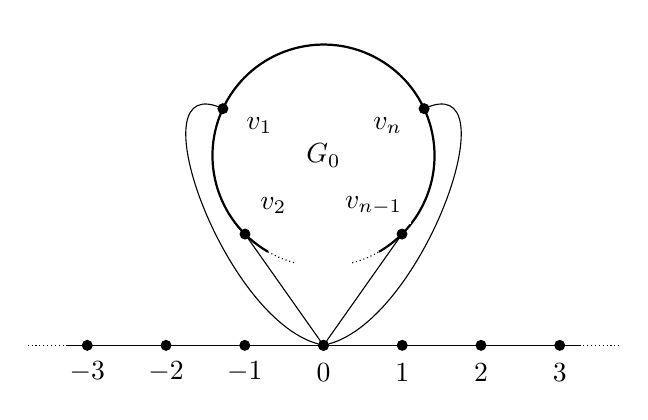
\begin{tikzpicture}[
  label distance=-5.5pt,
  thin,
  vertex/.style={circle,draw=black,fill=black,inner sep=1.25pt,
    minimum size =0mm},
  attach/.style={circle,draw=black,fill=white,inner sep=1.25pt,
    minimum size =0mm},
  dots/.style={circle,fill=black,inner sep=.5pt,
    minimum size= 0pt}]

% Path and Labels    
  \draw (-3.25,-2.41) -- (3.25,-2.41);
  
  \foreach \x in {-3,...,3}{
    \node at (\x,-2.41) [vertex] {};
    \node at (\x,-2.75) {$\x$};
  }
    
  \node (a) at (0,-2.41) [vertex] {};
  
  \draw[densely dotted] (-3.25,-2.41) -- (-3.75, -2.41);
  \draw[densely dotted] (3.25, -2.41) -- (3.75, -2.41);
  
% Graph  
  \draw[thick] (240:1.41) arc (240:-60:1.41);
  \draw[densely dotted] (240:1.41)  arc (240:255:1.41);
  \draw[densely dotted] (285:1.41)  arc (285:300:1.41);
  
  \foreach \i / \n /\t in {25 / n/ 15, 155 / 1/ 165, 225/ 2 / 120, 315 / {n-1}/60}{
    \node at (\i : .9) [rectangle,fill=white] {$v_\n$};
    \node at (\i : 1.41) [vertex] {};
  }
  \node at (0,0) [rectangle,fill=white] {$G_0$};

% Attaching Edges
  \foreach \i /\t in {25/15, 155/165}{
    \draw (\i:1.41) to[out=\i,in=\t] (a);
  }
  
  \foreach \i \in in {225,315}{
    \draw (\i:1.41) to (a);
  }

\end{tikzpicture}
  \caption{A simple example for graph scattering.  A graph $\widetilde{G}$ is attached to an infinite path.}
  \label{fig:path_and_graph}
\end{figure}

With this assumption, we can see that there are three distinct cases for the form of the eigenstates.  In particular, the eigenstate could have no amplitude along the infinite paths, being confined to the finite graph $\widehat{G}$.  It could also be a normalizable state not confined to the finite graph $\widehat{G}$, in that the amplitude along the infinite paths decays exponentially.  Finally, the eigenstate could be an unnormalizable state, in which case we will call it a scattering state.

In the first case, where the state is confined to the graph $\widetilde{G}$, we 



Let us finally assume that the state is a scattering state.  Note that the eigenvalue of the state must be between $[-2,2]$, and that the form of the eigenstate along the paths must be scalar multiples of $e^{ikx}$ and $e^{-ikx}$.  Explicitly, the state must be of the form
\begin{align}
  \braket{x}{\psi} = \begin{cases} A_k e^{i k x} + B_k e^{i k x} & x \leq 0\\
   C_k e^{i k x} + D_k e^{i k x} & x\geq 0\end{cases}
\end{align}
where we note that the amplitude can change at $x=0$ since we have attached the graph $\widetilde{G}$.  However, we do have that $A_k + B_k=C_k +D_k$, since the amplitude at $0$ is single valued.  Additionally, we have that the eigenvalue of this state is given by $2\cos(k)$.  Note that we have not yet determined the form of the eigenstate inside the graph $\widetilde{G}$, but if we define $\ket{\phi}$ to be the restriction of $\ket{\psi}$ to the finite graph $\widetilde{G}$, then $\ket{\phi}$ must satisfy the equation
\begin{equation}
  A(G) \ket{\phi} + (A_k + B_k)\sum_{v\in S} \ket{v}\braket{v}{\phi} = 2\cos(k) \ket{\phi},
\end{equation}
where the additional term arises from the fact that the vertices in $S$ are connected to the vertex $0$.  Finally, we have that
\begin{equation}
  2 \cos(k)\braket{0}{\psi} = Ae^{-ik} + B_k e^{ik} + C_k e^{i k} + D_k e^{-ik} + \sum_{v\in S} \braket{v}{\phi},
\end{equation}
since the eigenvalue equation must be satisfied at $0$.


We will focus on the case where $A_k = 1$ and $D_k=0$ and the case where $A_k = 0$ and $D_k=1$ individually, as they can each be thought of as a particle with momentum $k$ traveling toward the attached graph $\widetilde{G}$ along the infinite path, and then scattering.  Explicitly, if we first look at the case where $A_k = 1$ and $D_k = 0$,  we can see that
\begin{align}
  \braket{x}{\psi} = \begin{cases} e^{-ikx} + B_k e^{i kx} & x\leq 0\\
  C_k e^{-ikx} & x \geq 0\end{cases}
\end{align}
so that $1+ B_k  =C_k$.  Note that this is reminiscent of a scattering state, with reflection amplitude $B_k$ and transmission amplitude $C_k$, so that we take this intuition.  

\todo{make this coherent}




%%%%%%%%%%%%%%%
\subsection{General graphs}


More generally, let $\widehat{G}$ be any finite graph, with $n+m$ vertices and an adjacency matrix given by the block matrix
\begin{equation}
  A(\widehat{G}) = \begin{pmatrix}A & B^\dag\\ B & D\end{pmatrix},
\end{equation}
where $A$ is an $N\times N$ matrix, $B$ is an $m\times N$ matrix, and $D$ is an $m\times m$ matrix.  When examining graph scattering, we will be interested in the graph $G$ given by the graph-join of $\widehat{G}$ and $N$ semi-infinite paths, with an additional edge between each of the first $N$ vertices of $\widehat{G}$ and the first vertex of one semi-infinite path.  

We shall label label the first $N$ vertices of the graph $\widehat{G}$ as $(1,i)$, where $i\in[N]$, as these correspond to the first vertex in each semi-infinite path, and we will call these the \textit{terminal vertices}.  We refer to the other $m$ vertices of $\widehat{G}$ as the \textit{internal vertices} of $\widehat{G}$, and label them as $w\in[m]$, and we refer to the vertices on the $N$ semi-infinite paths as $(x,i)$, where $i\in[N]$ labels which infinite path the vertex is located on (corresponding to which vertex $(1,i)$ the path is attatched to), while $x\in \NN$ and $x\geq 2$ labels the distance along the semi-infinite path the vertex is located.  With this labeling of the vertices of $G$, the adjacency matrix of $G$ is then given by
\begin{equation}
  A(G) = A(\widehat{G}) + \sum_{j=1}^N \sum_{x=1}^\infty \big(\ketbra{x,j}{x+1,j} + \ketbra{x+1,j}{x,j}\big).
\end{equation}

At this point, we want to examine the possible eigenstates of the matrix $A(G)$.  It turns out that there are 3 different kinds of eigenstates, corresponding to the different qualitative properties of the eigenstate along the semi-infinite paths.

While we will mostly be interested in the third such type, it is important to understand the other kinds of eigenstates.

%%%%
\subsubsection{Confined bound states}

The easiest states to analyze are the confined bound states, which are eigenstates in which the only nonzero amplitudes are on vertices inside the finite graph $\widehat{G}$. If any vertex on the semi-infinite paths has nonzero amplitude for some eigenstate of the Hamiltonian, then the form of the Hamiltonian forces all vertices on that path to have nonzero amplitude, and thus these confined bound states are exactly those states that have finite support in the basis of vertex states.  

To find these confined bound states, we restrict our Hilbert space to the space spanned by the internal vertices of $\widehat{G}$. The states of interest then correspond to the eigenstates of $D$ (the induced adjacency matrix of $A(G)$ when restricted to the internal vertices of $\widehat{G}$) with the additional restriction that the state lies in the nullspace of $B^\dag$, so that we can extend this state to the full Hilbert space by simply assuming all other amplitudes are zero.    

As we originally assumed that there are only $m$ internal vertices of $\widehat{G}$, there are at most $m$ such confined bound states.  Additionally, note that there are no restrictions on the eigenvalues of these states, other than those that are inherited from any restrictions placed on it by $D$ (such as the energy being bounded by the maximum degree of $\widehat{D}$).

%%%%
\subsubsection{Unconfined bound states}

The next possible type of eigenstates are those that are not confined to the finite graph $\widehat{G}$ but are still normalizable.  Since these states still have amplitude along the semi-infinite paths, we know that they must be of the form $Ae^(i k x)$, for some $A$ and $k$.  However, when $k$ is not real (corresponding to a decaying amplitude along the paths), we have that
\begin{equation}
  2 \cos(k) = 2\cos(k_r + i k_i) = 2 \cos(k_r) \cosh(k_i) - i \sin(k_r) \sinh(k_i).
\end{equation}
Hence, if we assume that the state is normalizable, then $k_i \neq 0$, and as the adjacency matrix is Hermitian, we must have that the eigenvalue is real, forcing $k_r = \pi n$ for some $n\in \NN$.  Note that this then implies that $e^{i k} = z$, for some $z\in(-1,1)\setminus\{0\}$ (where $0$ corresponds to the confined bound states).

\todo{Finish this section, and determine whether this is  finite or infinite.}

%%%%
\subsubsection{Half-bound states}

The half-bound states are the limit of the states as $\kappa \rightarrow 0$.  In particular, they are those states where the amplitude along the infinite paths take the form $(\pm 1)^x$.  These states aren't quite bound, in that they are not normalizable, but they are also not quite scattering states, as they correspond to non-moving scattering states.  They won't play much of a role in this paper, but I did want to mention them.

%%%%
\subsubsection{Scattering states}

We finally reach the point of scattering states, or those states we can use for computational tasks.  We first assume that we are orthogonal to all bound states, and in particular that we are othogonal to all confined bound states.  This allows us to uniquely construct the scattering states (without this assumption, if there existed a confined bound state at the appropriate energy, then we could simply add any multiple of the confined bound state to get a different scattering state).

Taking some intuition from the classical case, we will construct a set of states that correspond to sending a particle in towards the graph $\widehat{G}$ along one of the semi-infinite paths and understanding how it scatters off of the graph.  Namely, for each $i\in[N]$ we will assume that there exists a state with amplitude along the $i$-th path of the form $e^{i k x} + S_{i,i}(k)e^{-i k x}$ for $k\in (-\pi, 0)$, and that the rest of the paths have amplitudes given by $S_{i,q}(k)e^{ikx}$.  More concretely, we assume that the form of the states is given on the infinite paths by
\begin{equation}
  \braket{x,q}{\scat_{j}(k)} = \delta_{j,q} e^{-i k x} + S_{qj} e^{i k x}.
\end{equation}
We then need to see whether such an eigenstate exists.  In this case, note that $S_{qj}$ corresponds to the transmitted amplitude along the $q$-th path if the particle was incident along the $j$-th path.

If we continue to make the assumption that these states exist, we can also write the amplitudes of the $m$ interval vertices as a column vector, as $\vec{\psi}_i(k)$, in which $\vec{\psi}_{i(k)}$ is the projection of $\ket{\scat_j(k)}$ onto the internal vertices of $\widehat{G}$.  We can then collect these vectors into an $N\times m$ matrix, namely
\begin{equation}
  \Psi(k) := \begin{pmatrix} \vec{\psi}_1(k) & \vec{\psi}_2(k) & \cdots & \vec{\psi}_N(k)\end{pmatrix}
\end{equation}
\todo{check if this is correct $N\times m$ or $m\times N$}

Noting that the amplitudes for $\vec{\scat_j(k)}$ on the terminal vertices is given by $ e^{-i k} \ket{1,j} + S_{j}(k)e^{ik}$ (thinking of $S_{j}(k)$ as a vector), we can then collect all of the eigenvalue equations for the vertices in $\widehat{G}$ (both internal and termal) as
\begin{equation}
  \begin{pmatrix} A & B^\dag \\
    B & D\end{pmatrix} \begin{pmatrix}  e^{-i k} \II + S(k) e^{i k}\\ \Psi(k)\end{pmatrix} 
    + \begin{pmatrix} e^{-2 i k} \II + e^{2 i k} S(k)\\ 0\end{pmatrix} = 
    2 \cos(k) \begin{pmatrix}  e^{-i k} \II + S(k) e^{i k}\\ \Psi(k)\end{pmatrix}.
\end{equation}

By examining the lower half of this matrix equation, we can see that
\begin{equation}
  \Psi(z) = \frac{1}{2 \cos(k) \II - D} \big( e^{-ik} B + e^{i k} B S(z)\big),
\end{equation}
which gives the amplitudes of the internal vertices in terms of the scattering matrix.

If we then examine the upper half of the matrix equation, we find that
\begin{align}
  A\big(e^{-ik} \II+ e^{i k} S(k)\big) + B^\dag \Psi(k) + \big(e^{-2 ik}\II + e^{2 i k} S(z)\big) &= 2 \cos(k) \big(e^{-ik} \II + e^{i k} S(k)\big)&\Rightarrow\\
  -\Bigg(\II - e^{ik}\Big(A + B^\dag \frac{1}{2 \cos(k) - D} B\Big)\Bigg)S(k) &= \II - e^{-ik}\Big(A + B^\dag \frac{1}{2 \cos(k) - D} B\Big).
\end{align}
Hence, if we define
\begin{equation}
  Q(k) = \II - e^{ik}\Big( A + B^\dag \frac{1}{2 \cos(k) - D} B\Big),
\end{equation}
we find that
\begin{equation}
  S(k) = - Q(k)^{-1} Q(-k).
\end{equation}

Putting this all together, we then have that the states $\ket{\scat_j(k)}$ exist for all $k$ in which the matrix operations defining $S(k)$ are well defined.  In particular, we take the inverse of $2\cos(k)\II - D$, and the inverse of $Q(k)$.  These only possibly have problems when 

%%%%
\subsubsection{Easier calculation of $S$-matrix}
\todo{come up with a better name of this cycle}


While the above is useful for most values of $k\in(-pi,0)$, unfortunately there are specific values of $k$ (such as those for which $D$ has eigenvalue $2\cos(k)$) in which the above analysis doesn't hold do to the singularity of some particular matrices.  If we want to show that these scattering states exist for all $k\in (-\pi,0)$, we need to somehow show that these singularities are just a problem of the analysis and are not intrinsic barriers to existence.

Along these lines, let us extend our analysis to complex $z$, instead of only focusing on the real line.  As such, let us define the matrix
\begin{equation}
  \gamma(z) := \begin{pmatrix}  z A - \II & z B^\dag\\
    z B & zD - (1+z^2) \II\end{pmatrix}.
    \label{eq:gamma_def}
\end{equation}

Note that 
\begin{align}
  \begin{pmatrix} \II & zB^\dag\\
    0 & z D - (1+ z^2) \II \end{pmatrix}
    \begin{pmatrix} - Q(z) & 0\\
      \frac{z}{zD - (1+ z^2)\II}B & \II\end{pmatrix} 
      &= \begin{pmatrix} -Q(z) + z B^\dag \frac{1}{D - (z + z^{-1})} B & z B^\dag\\
        zB & zD - (1+z^2)\II\end{pmatrix} \\
        &= \gamma(z)
\end{align}
Additionally, if we note that the inverse of a block diagonal matrix can be written as
\begin{equation}
  \begin{pmatrix} X & Y \\
  Z & W\end{pmatrix}^{-1} = \begin{pmatrix} \big(X - Y W^{-1} Z\big)^{-1} & - X^{-1} Y \big(W - Z X^{-1} Y\big)^{-1}\\
    - W^{-1} Z \big(X - Y W^{-1} Z\big)^{-1} & \big(W - Z X^{-1} Y\big)^{-1}\end{pmatrix},
\end{equation}
then we can see that
\begin{align}\gamma(z)^{-1} &= \begin{pmatrix} - Q(z) & 0\\
      \frac{z}{zD - (1+ z^2)\II}B & \II\end{pmatrix}^{-1} \begin{pmatrix} \II & zB^\dag\\
    0 & z D - (1+ z^2) \II \end{pmatrix}^{-1}\\
    &= \begin{pmatrix}
      - Q(z)^{-1} & 0\\
      \frac{z}{z D - (1+z^2)\II} B Q(z)^{-1} & \II
    \end{pmatrix}
    \begin{pmatrix}
      \II & - B^{\dag} \frac{z}{zD - (1+z^2)\II}\\
      0 & \frac{1}{zD - (1+z^2)\II}
    \end{pmatrix}.
\end{align}
We can then use this to see that
\begin{align}
  \gamma (z)^{-1} \gamma(z^{-1}) &= \begin{pmatrix}
      - Q(z)^{-1} & 0\\
      \frac{z}{z D - (1+z^2)\II} B Q(z)^{-1} & \II
    \end{pmatrix}
    \begin{pmatrix}
      \II & - B^{\dag} \frac{z}{zD - (1+z^2)\II}\\
      0 & \frac{1}{zD - (1+z^2)\II}
    \end{pmatrix}
    \begin{pmatrix} \II & z^{-1}B^\dag\\
    0 & z^{-1} D - (1+ z^{-2}) \II \end{pmatrix}
    \begin{pmatrix} - Q\big(z^{-1}\big) & 0\\
      \frac{z^{-1}}{z^{-1}D - (1+ z^{-2})\II}B & \II\end{pmatrix} \\
  &=  \begin{pmatrix}
      - Q(z)^{-1} & 0\\
      \frac{z}{z D - (1+z^2)\II} B Q(z)^{-1} & \II
    \end{pmatrix}
    \begin{pmatrix}
      \II & 0\\
      0 &z^{-2}\II \end{pmatrix}
    \begin{pmatrix} - Q\big(z^{-1}\big) & 0\\
      \frac{z^{-1}}{z^{-1}D - (1+ z^{-2})\II}B & \II\end{pmatrix} \\
   &= \begin{pmatrix}
      - Q(z)^{-1} & 0\\
      \frac{z}{z D - (1+z^2)\II} B Q(z)^{-1} &z^{-2} \II
    \end{pmatrix}
    \begin{pmatrix} - Q\big(z^{-1}\big) & 0\\
      \frac{z^{-1}}{z^{-1}D - (1+ z^{-2})\II}B & \II\end{pmatrix} \\
  &= \begin{pmatrix}
      Q(z)^{-1}Q(z^{-1}) & 0\\
      \frac{1}{D - (z+z^{-1})\II }B \big(z^{-2} \II - Q(z)^{-1}Q(z^{-1}) \big) & z^{-2}\II
    \end{pmatrix}\\
  &= -\begin{pmatrix}
      S(z) & 0\\
     z^{-1} \Psi(s) & -z^{-2}\II
    \end{pmatrix}\label{eq:gamma_gives_S}
\end{align}

As such, we can write we have a nice representation of the scattering matrix and the interior amplitudes in terms of the matrix $\gamma$.  If we then note that
\begin{equation}
  \gamma(z)^{-1} = \frac{1}{\det \gamma(z)} \adj \gamma (z)
\end{equation}
where $\adj \gamma (z)$ is the adjugate matrix of $\gamma(z)$, then by \eq{gamma_gives_S} we can then see that the entries of $S(z)$ are rational functions of $z$. 

\todo{this still doesn't explain why we can define the S-matrix this way when things aren't invertable explanation}

%%%%%%%%%%%%%%%
\subsection{Scattering matrix properties}

While the use of the $\gamma$ matrix gives an explicit construction of the form of the eigenstates on the internal vertices, it is also useful to note that the scattering matrix at a particular momentum $k$ can be expressed as
\begin{equation}
  S(k) = - Q(z)^{-1} Q(z^{-1}),
\end{equation}
where $z=e^{i k}$, and the matrices $Q(z)$ are given by
\begin{equation}
  Q(z) = \II - z \Big( A + B^\dag \frac{1}{ \frac{1}{z} + z - D} B\Big).
\end{equation}
Note that $Q(z)$ and $Q(z^{-1})$ commute for all $z\in \CC$, as they can both be written as $\II + z H(z + z^{-1})$.

Using this expression for the scattering matrix, it is easy to see that $S(k)$ is a unitary matrix, as 
\begin{equation}
  S(k)^{\dag} = - Q(z^{-1})^\dag (Q(z)^{-1})^\dag
\end{equation}
and that
\begin{equation}
  Q(z)^\dag = \II^\dag - z^\dag\Big( A^\dag + B^\dag \Big(\frac{1}{\frac{1}{z} + z - D}\Big)^\dag (B^\dag)^\dag\Big) 
     = \II - z^\dag \Big(A + B^\dag \frac{1}{\frac{1}{z^\dag} + z^\dag - D} B \Big) = Q(z^\dag)
\end{equation}
and thus
\begin{equation}
  S(k)^\dag = -Q(z^{-1})^\dag (Q(z)^{-1})^\dag = - Q(z) Q(z^{-1})^{-1} = Q(z^{-1})^{-1} Q(z) = S(k)^{-1}
\end{equation}
where we used the fact that $z=e^{ik}$ so that $z^\dag = z^{-1}$, and the fact that $Q(z)$ and $Q(z^{-1})$ commute.

Additionally, we can make use of the fact that $S$ is derived from an unweighted graph to show that the scattering matrices are symmetric.  In particular, note that $Q(z)$ is symmetric for all $z$, since $D$ is symmetric, symmetric matrices are closed under inversion, $A$ is symmetric and $B$ is a 0-1 matrix.  As such, we have that
\begin{align}
  S(k)^T &= -\big( Q(z)^{-1} Q(z^{-1})\big)^T = -Q(z^{-1})^T (Q(z)^{-1})^T \\
    &= -Q(z^{-1}) Q(z)^{-1} = -Q(z)^{-1} Q(z^{-1}) = S(k)
\end{align}
where we used the fact that $Q(z)$ and $Q(z^{-1})$ commute.

Putting this together, we have that $S(k)$ is a symmetric, unitary matrix for all $k$.

%%%%%%%%%%%%%%%%%
\subsection{Orthonormality of the scattering states}

\todo{go over this section more}

We now establish the delta-function normalization of the scattering states. Let 
\begin{align*}
\Pi_{1} & = \sum_{x=1}^{\infty}\sum_{q=1}^{N}|x,q\rangle\langle x,q|\\
\Pi_{2} & = \mathbb{I}-\sum_{x=2}^{\infty}\sum_{q=1}^{N}|x,q\rangle\langle x,q|\\
\Pi_{3} & = \sum_{q=1}^{N}|1,q\rangle\langle1,q|.\end{align*}
We show that, for $k\in(-\pi,0)$, $p\in(-\pi,0)$, and $i,j\in\{1,\ldots,N\}$,
\begin{equation}
\langle\mathrm{sc}_{i}(p)|\mathrm{sc}_{j}(k)\rangle=\langle\mathrm{sc}_{i}(p)|\Pi_{1}+\Pi_{2}-\Pi_{3}|\mathrm{sc}_{j}(k)\rangle=2\pi\delta_{ij}\delta(k-p).\label{eq:delta}\end{equation}
First write 
\begin{align*}
\langle\mathrm{sc}_{i}(p)|\Pi_{1}|\mathrm{sc}_{j}(k)\rangle & = \sum_{x=1}^{\infty}\sum_{q=1}^{N}(\delta_{iq}e^{ipx}+S_{qi}^{\ast}(p)e^{-ipx})(\delta_{jq}e^{-ikx}+S_{qj}(k)e^{ikx})\\
 & = \frac{1}{2}\left(\delta_{ij}+\sum_{q=1}^{N}S_{qi}^{\ast}(p)S_{qj}(k)\right)\left(\sum_{x=1}^{\infty}e^{i(p-k)x}+\sum_{x=1}^{\infty}e^{-i(p-k)x}\right)\\
 & \quad +\frac{1}{2}\left(\delta_{ij}-\sum_{q=1}^{N}S_{qi}^{\ast}(p)S_{qj}(k)\right)\left(\sum_{x=1}^{\infty}e^{i(p-k)x}-\sum_{x=1}^{\infty}e^{-i(p-k)x}\right)\\
 & \quad +\frac{1}{2}(S_{ji}^{\ast}(p)+S_{ij}(k))\left(\sum_{x=1}^{\infty}e^{-i(p+k)x}+\sum_{x=1}^{\infty}e^{i(p+k)x}\right)\\
 & \quad +\frac{1}{2}(S_{ji}^{\ast}(p)-S_{ij}(k))\left(\sum_{x=1}^{\infty}e^{-i(p+k)x}-\sum_{x=1}^{\infty}e^{i(p+k)x}\right).\end{align*}
We use the following identities for $p,k\in(-\pi,0)$: 
\begin{align*}
\sum_{x=1}^{\infty}e^{i(p-k)x}+\sum_{x=1}^{\infty}e^{-i(p-k)x} & = 2\pi\delta(p-k)-1 \\
\sum_{x=1}^{\infty}e^{i(p+k)x}+\sum_{x=1}^{\infty}e^{-i(p+k)x} &=-1 \\
\sum_{x=1}^{\infty}e^{i(p-k)x}-\sum_{x=1}^{\infty}e^{-i(p-k)x} & = i\cot\left(\frac{p-k}{2}\right) \\
\sum_{x=1}^{\infty}e^{i(p+k)x}-\sum_{x=1}^{\infty}e^{-i(p+k)x} &= i\cot\left(\frac{p+k}{2}\right).
\end{align*}
These identities hold when both sides are integrated against a smooth function of $p$ and $k$. Substituting, we get
\begin{align}
\langle\mathrm{sc}_{i}(p)|\Pi_{1}|\mathrm{sc}_{j}(k)\rangle & =  2\pi\delta_{ij}\delta(p-k)+\delta_{ij}\left(\frac{i}{2}\cot\left(\frac{p-k}{2}\right)-\frac{1}{2}\right)\nonumber\\
&\quad+\sum_{q=1}^{N}S_{qi}^{\ast}(p)S_{qj}(k)\left(-\frac{i}{2}\cot\left(\frac{p-k}{2}\right)-\frac{1}{2}\right)\nonumber \\
 &\quad+S_{ji}^{\ast}(p)\left(-\frac{1}{2}-\frac{i}{2}\cot\left(\frac{p+k}{2}\right)\right)\nonumber\\
&\quad+S_{ij}(k)\left(-\frac{1}{2}+\frac{i}{2}\cot\left(\frac{p+k}{2}\right)\right)\label{eq:pi1}
\end{align}
where we used unitarity of the $S$-matrix to simplify the first term.
Now turning to $\Pi_{2}$ we have \[
\langle\mathrm{sc}_{i}(p)|H\Pi_{2}|\mathrm{sc}_{j}(k)\rangle=2\cos(p)\langle\mathrm{sc}_{i}(p)|\Pi_{2}|\mathrm{sc}_{j}(k)\rangle\]
 and 
\begin{align*}
\langle\mathrm{sc}_{i}(p)|H\Pi_{2}|\mathrm{sc}_{j}(k)\rangle & = \langle\mathrm{sc}_{i}(p)|\bigg(2\cos(k)\Pi_{2}|\mathrm{sc}_{j}(k)\rangle+\sum_{q=1}^{N}(e^{-ik}\delta_{qj}+S_{qj}(k)e^{ik})|2,q\rangle\\
&\quad -\sum_{q=1}^{N}(e^{-2ik}\delta_{qj}+S_{qj}(k)e^{2ik})|1,q\rangle\bigg).
\end{align*}
 Using these two equations we get 
\begin{align*}
(2\cos(p)-2\cos(k))\langle\mathrm{sc}_{i}(p)|\Pi_{2}|\mathrm{sc}_{j}(k)\rangle & =  \delta_{ij} (e^{2ip-ik}-e^{-2ik+ip})+S_{ji}^{\ast}(p)(e^{-2ip-ik}-e^{-2ik-ip})\\
 & \quad +S_{ij}(k)(e^{2ip+ik}-e^{2ik+ip})\\
& \quad +\sum_{q=1}^{N}S_{qi}^{\ast}(p)S_{qj}(k)(e^{-2ip+ik}-e^{2ik-ip}).
\end{align*}
 Noting that
\[
\langle\mathrm{sc}_{i}(p)|\Pi_{3}|\mathrm{sc}_{j}(k)\rangle=\sum_{q=1}^{N}(\delta_{iq}e^{ip}+S_{qi}^{\ast}(p)e^{-ip})(\delta_{jq}e^{-ik}+S_{qj}(k)e^{ik}),
\]
we have 
\begin{align}
\langle\mathrm{sc}_{i}(p)|\Pi_{2}-\Pi_{3}|\mathrm{sc}_{j}(k)\rangle & = \delta_{ij}\left(\frac{e^{2ip-ik}-e^{-2ik+ip}}{2\cos(p)-2\cos(k)}-e^{ip-ik}\right)\nonumber\\
&\quad+S_{ji}^{\ast}(p)\left(\frac{e^{-2ip-ik}-e^{-2ik-ip}}{2\cos(p)-2\cos(k)}-e^{-ip-ik}\right)\nonumber \\
 & \quad +S_{ij}(k)\left(\frac{e^{2ip+ik}-e^{2ik+ip}}{2\cos(p)-2\cos(k)}-e^{ip+ik}\right)\nonumber\\
&\quad+\sum_{q=1}^{N}S_{qi}^{\ast}(p)S_{qj}(k)\left(\frac{e^{-2ip+ik}-e^{2ik-ip}}{2\cos(p)-2\cos(k)}-e^{-ip+ik}\right)\nonumber \\
  & = \delta_{ij}\left(\frac{1}{2}-\frac{i}{2}\cot\left(\frac{p-k}{2}\right)\right)+S_{ji}^{\ast}(p)\left(\frac{1}{2}+\frac{i}{2}\cot\left(\frac{p+k}{2}\right)\right)\nonumber\\
&\quad+S_{ij}(k)\left(\frac{1}{2}-\frac{i}{2}\cot\left(\frac{p+k}{2}\right)\right)\nonumber\\
&\quad+\sum_{q=1}^{N}S_{qi}^{\ast}(p)S_{qj}(k)\left(\frac{1}{2}+\frac{i}{2}\cot\left(\frac{p-k}{2}\right)\right).
\label{eq:pi2_pi3}
\end{align}
 Adding equation \eq{pi1} to equation \eq{pi2_pi3} gives
equation \eq{delta}.

\todo{These form an orthonormal basis if you also include the bound states, but this is Theorem 1 from Andrew and David's Levison's Theorem II paper.  I'm not sure if I should include it.}

\section{Applications of graph scattering}

\subsection{NAND Trees}

The motivating idea for understanding graph scattering was an explicit algorithm that computes the value of a NAND tree with $N$ leaves in $\OO(\sqrt{N})$ time.  In particular, a NAND tree is a complete binary tree of depth $\log N$, where each leaf has a particular binary value.  Each node of the tree is then assigned a binary value by evaluating the NAND of its children, and the value of the entire tree is the value of the root node.  Classically, any randomized algorithm requires $\OO(N^{0.753})$ queries to the roots in order to evaluate the value of the tree, and thus this gives an example of a quantum speedup.

The reason that we are interested in this is that the original algorithm uses graph scattering as the actual algorithm.  In particular, a binary tree is attached to an infinite path at the root, and then additional vertices are attached to the leaves depending on whether the binary value is 0 or 1.  It turns out that at energy 0 (i.e., momentum $-\pi/2$), such a tree has perfect transmission from one path to the other if the tree evaluates to 1, and perfect reflection if the tree evaluates to 0.  Hence, if a wave packet with momentum centered around $-\pi/2$ is scattered off of such a graph, then if we determine the location of the particle after it has scattered we evaluate the tree. 

In this case, the requisite size of the wavepacket turns out to be $\OO(\sqrt{N})$, and thus this amount of time is required in order for the scattering to occur.  This is closely related to the number of queries to the values of the input variables in order to compute the value of the tree, and thus this is a quantum algorithm that has a provable speedup over classical computing.

\subsection{Momentum dependent actions}

While the NAND trees gives a good example of how the process works, in that the scattering evaluates a binary function, we can use similar ideas in order to have nontrivial scattering behavior.  In particular, the NAND tree algorithm utilizes the fact that some graph either completely reflects or transmits at one particular momenta in order to evaluate the function, but we can also create graphs that have different behaviors at different momenta, or that perfectly transmits to some subset of the attached paths (i.e., generalizations to multiple semi-infinite paths).

%%%%%%%%%%%%%%%%%%%%%%%%%%%%%%%%%%%%%%%%%%%%%%%%%%%%%%%%%%%%%%%%%

\subsubsection{R/T gadets}

The easiest thing we could hope for are exactly similar to the NAND trees experiment, in that if there are only two attached semi-infite paths, then at some fixed momenta it either completely transmits, or it completely reflects.  However, in contrast to the NAND tree, we will only work with a single graph, and use it to filter out some momenta.

Basically, the idea behind R/T gadgets is to perfectly transmit at some momenta, while perfectly reflecting at other momenta.  This will then allow us to filter out certain unwanted wavepackets, and allow us to only deal with the momenta of interest.  Further, these simple gadgets can be used as a simple building block in the construction of other graphs, allowing us to have more complicated graphs.

%%%%%%%%%%%%%%%%%%%%%%%%%%%%%%%%%%%%%%%%%%%%%%%%%%%%%%%%%%%%%%%%%

\subsubsection{Momentum Switches}

In addition to a simple graph that only reflects or transmits certain momenta, we can generalize the idea to a kind of routing behavior.  In particular, we can attempt to construct a graph with three attached semi-infinite paths, in which when a wavepacket is incident on one particular path, it either perfectly transmits to the second path, or it perfectly transmits to the third path, depending on the incident momenta.  In this way, we construct something like a momentum dependent railroad switch, sending different wavepackets to different locations.

In the grand scheme of things, this is extremely useful, as it allows for more general momentum dependent actions.

%%%%%%%%%%%%%%%%%%%%%%%%%%%%%%%%%%%%%%%%%%%%%%%%%%%%%%%%%%%%%%%%%

\subsection{Encoded unitary}

Finally, we can also encode unitary actions using these graphs, in that by necessity these scattering matrices must be unitary.  In particular, let us examine what happens to a graph with four attached semi-infinite paths, when at some chosen momentum a wavepacket from either of the first two paths gets perfectly transmits to the last two paths.  In this case, the S-matrix becomes a block matrix, with the two $2\times 2$ blocks in the diagonal both zero matrices.  As such, the off diagonal matrices must also be unitary, and if we think of the two input paths as an encoded qubit (with a wavepacket along one path corresponding to an encoded $\ket{0}$ state and a wavepacket along the other path correpsonding to an encoded $\ket{1}$ state) then this scattering procedure performs some encoded unitary transformation on the qubit.


%%%%%%%%%%%%%%%%%%%%%%%%%%%%%%%%%%%%%%%%%%%%%%%%%%%%%%%%%%%%%%%%%
%  Constructing graphs
%%%%%%%%%%%%%%%%%%%%%%%%%%%%%%%%%%%%%%%%%%%%%%%%%%%%%%%%%%%%%%%%%

\section{Construction of graphs with particular scattering behavior}

While we have shown that the scattering behavior of some given graph is easy to compute, finding a graph with a given scattering behavior is much more difficult.  We don't even know whether such an operation is decidable, and thus constructing an efficient algorithm for finding a graph with a given scattering behavior seems unlikely.  However, there are specific behaviors at particular momenta in which constructions are known, and some small sized graphs that have been found via exhaustive searches.


%%%%%%%%%%%%%%%%%%%%%%%%%%%%%%%%%%%%%%%%%%%%%%%%%%%%%%%%%%%%%%%%%

\subsection{R/T gadgets}

\todo{Go over this section, and revise}

Perhaps the most simple behavior will be two-terminal gadgets that either perfectly reflect at some particular momenta, or perfectly transmit.  While this is still a rather complicated problem when the terminals can be any vertices of the graph, things become tractable when we want to only attach a graph to a single vertex of an infinite path.  In this case, everything works out as expected.

We refer to the graph shown in \fig{reversal_orig} as $\hat{G}$, and we write $G$ for the full graph obtained by attaching two semi-infinite paths to terminals $(1,1)$ and $(1,2)$.  As shown in the Figure, the graph $\hat{G}$ for a type 1 gadget is determined by a finite graph $G_0$ and a subset $P = \{p_1,\ldots,p_n\} \subseteq V(G_0)$ of its vertices, called the \emph{periphery}.  Each vertex in the periphery is connected to a vertex denoted $a$, and $a$ is also connected to two terminals $(1,1)$ and $(1,2)$. A type 1 R/T gadget with $n=1$ has only one edge between $G_0$ and $a$; in this special case we also call it a \emph{type 2 R/T gadget} (see \fig{reversalRT}).

Looking at the eigenvalue equation for the scattering state $\ket{\sc_{1} (k)}$ at vertices $(1,1)$ and $(1,2)$, we see that the amplitude at vertex $a$ satisfies
\[
  \langle{a}\ket{\sc_{1} (k)} = 1 + R(k) = T(k).
\] 
Thus perfect reflection at momentum $k$ occurs if and only if $R(k)=-1$ and $\langle{a}\ket{\sc_{1} (k)}=0$, while perfect transmission occurs if and only if $T(k)=1$ and $\langle{a}\ket{\sc_{1} (k)}=1$. Using this fact, we now derive conditions on the graph $G_0$ that determine when perfect transmission and reflection occur.

For type 1 gadgets, we give a necessary and sufficient condition for perfect reflection: $G_0$ should have an eigenvector for which the sum of amplitudes on the periphery is nonzero.

\begin{lemma}\label{lem:reflect_reqs}
Let $\hat{G}$ be a type 1 R/T gadget. A momentum $k\in (-\pi,0)$ is in the reflection set $\mathcal{R}$ if and only if $G_0$ has an eigenvector $\ket{\chi_k}$ with eigenvalue $2\cos(k)$ satisfying
\begin{equation}
  \sum_{i=1}^{n} \braket{p_i}{\chi_k} \neq 0. \label{eq:sum_condition}
\end{equation}
\end{lemma}

\begin{proof}
First suppose that $\hat{G}$ has perfect reflection at momentum $k$, i.e., $R(k)=-1$ and $\langle{a}\ket{\sc_{1} (k)}=0$. Since $\langle{(1,1)}\ket{\sc_1(k)} = e^{-ik} - e^{ik}\neq 0$ and $\langle{(1,2)}\ket{\sc_1(k)}=0$, to satisfy the eigenvalue equation at vertex $a$, we have
\[
  \sum_{j=1}^{n} \langle{p_j}\ket{\sc_1(k)} = e^{ik} - e^{-ik} \neq 0.
\]
Further, since $G_0$ only connects to vertex $a$ and the amplitude at this vertex is zero, the restriction of $\ket{\sc_1(k)}$ to $G_0$ must be an eigenvector of $G_0$ with eigenvalue $2\cos(k)$. Hence the condition is necessary for perfect reflection. 
 
Next suppose that $G_0$ has an eigenvector $\ket{\chi_k}$ with eigenvalue $2\cos(k)$ satisfying \eq{sum_condition}, with the sum equal to some nonzero constant $c$. Define a scattering state $\ket{\psi_k}$ on the Hilbert space of the full graph $G$ with amplitudes
\[
  \braket{v}{\psi_k} = \frac{e^{ik} - e^{-ik}}{c} \braket{v}{\chi_k}
\]
for all $v \in V(G_0)$, $\braket{a}{\psi_k}=0$, and 
\[
 \braket{(x,j)}{\psi_k}=\begin{cases} e^{-ikx}-e^{ikx} & j=1\\
0 & j=2
\end{cases}
\]
for all $x \in \posint$.

We claim that $\ket{\psi_k}$ is an eigenvector of $G$ with eigenvalue $2 \cos(k)$.  The state clearly satisfies the eigenvalue equation on the semi-infinite paths since it is a linear combination of states with momentum $\pm k$.  At vertices of $G_0$, the state is proportional to an eigenvector of $G_0$, and since the state as no amplitude at $a$, the eigenvalue equation is also satisfied at these vertices.  It remains to see that the eigenvalue equation is satisfied at $a$, but this follows immediately by a simple calculation.

Since $\ket{\psi_k}$ has the form of a scattering state with perfect reflection, we see that $R(k)=-1$ and $T(k)=0$ as claimed.
\end{proof}

The following Lemma gives a sufficient condition for perfect transmission (which is also necessary for type 2 gadgets).  Let $g_0$ denote the induced subgraph on $V(G_0)\setminus P$ where $P = \{p_i\colon i\in [n]\}$ is the periphery.

\begin{lemma}\label{lem:transmit_reqs}
Let $\hat{G}$ be a type 1 R/T gadget and let $k\in (-\pi,0)$. Suppose $\ket{\xi_k}$ is an eigenvector of $g_0$ with eigenvalue $2\cos{k}$ and with the additional property that, for all $i \in [n]$,
\begin{equation}
\label{eq:trans_cond}
  \sum_{\substack{v \in V(g_0): \\ (v,p_i)\in E(G_0)}} \braket{v}{\xi_k} = c \neq 0 
\end{equation}
for some constant $c$ that does not depend on $i$. Then $k$ is in the transmission set $\mathcal{T}$. If $\hat{G}$ is a type 2 R/T gadget, then this condition is also necessary.
\end{lemma}

\begin{proof}
If $g_0$ has a suitable eigenvector $\ket{\xi_k}$ satisfying \eq{trans_cond}, define a scattering state $\ket{\psi_k}$ on the full graph $G$, with amplitudes $\langle a\ket{\psi_k}=1$, 
\begin{equation}
  \braket{v}{\psi_k} 
  = \begin{cases} -\frac{1}{c} \braket{v}{\xi_k} & v\in V(g_0)\\
  	0 & v \in P
\end{cases}
\label{eq:psik_c}
\end{equation}
in the graph $G_0$, and 
\[
 \langle{(x,j)} \ket{\psi_k}=\begin{cases} e^{-ikx} & j=1\\
 e^{ikx} & j=2
\end{cases}
\]
for $x \in \posint$.  As in the proof of \lem{reflect_reqs}, the state $\ket{\psi_k}$ is clearly satisfies the eigenvalue equation (with eigenvalue $2\cos(k)$) at vertices on the semi-infinite paths and vertices of $g_0$.  The factor of $-\frac{1}{c}$ in \eq{psik_c} is chosen so that the eigenvalue condition is satisfied at vertices in $P$.  It is easy to see that the eigenvalue condition is also satisfied at $a$.

Since $\ket{\psi_k}$ is a scattering eigenvector of $G$ with eigenvalue $2\cos(k)$ and perfect transmission, we have $T(k)=1$.

Now suppose $\hat{G}$ is a type 2 R/T gadget (as shown in \fig{reversalRT}), with $P = \{p\}$.  Perfect transmission along with the eigenvalue equation at vertex $a$ implies
\[
\braket{p}{\sc_1(k)} = 0,
\]
so the restriction of $\ket{\sc_1(k)}$ to $g_0$ must be an eigenvector (since $p$ is the only vertex connected to $g_0$).  The eigenvalue equation at $p$ gives
\[
  \braket{a}{\sc_1(k)} 
  + \sum_{w \colon (w,p)\in E(G_0)} \braket{w}{\sc_1(k)} = 0 
  \quad\implies\quad
  \sum_{w \colon (w,p)\in E(G_0)} \braket{w}{\sc_1(k)} = -1.
\]
Hence the restriction of $\ket{\sc_1(k)}$ to $V(g_0)$ is an eigenvector of the induced subgraph, with the additional property that the sum of the amplitudes at vertices connected to $p$ is nonzero.
\end{proof}

%%%%%%%%%%
\subsubsection{Explicit constructions}

While the above gives a nice abstract explanation for the construction of R/T gadgets, it doesn't provide us with a concrete example without the graphs that satisfy the assumptions of the lemmas.  As such, let us look at two simple graphs.

As a first example, suppose $G_0$ is a finite path of length $l_1+l_2-2$ connected to $a$ at the $l_1$th vertex, as shown in \fig{RT_path}.  We determine the reflection and transmission sets as a function of $l_1$ and $l_2$.


%%%%%%%%%
\begin{figure}
  \centering
  \tikzsetnextfilename{GS_RT_path}
  \begin{tikzpicture}[
  thin,
  vertex/.style={circle,draw=black,fill=black,inner sep=1.25pt,
    minimum size =0mm},
  attach/.style={circle,draw=black,fill=white,inner sep=1.25pt,
    minimum size =0mm},
  dots/.style={circle,fill=black,inner sep=.5pt,
    minimum size= 0pt}]
    
    \draw (-1,-1) -- (1,-1);
    \draw (0,0) -- (0,-1);
    
    \node[attach,label=270:{$(1,1)$}] at (-1,-1) {};
    \node[attach,label=270:{$(1,2)$}] at (1,-1) {};
    \node[vertex,label={[label distance=.25*\baselineskip]270:{$ a $}},] at (0,-1) {};
    \node[vertex] at (0,0) {};
    
    % left branch
    \draw (0,0) -- (135:1.5);
    \draw[densely dotted] (135:1.5) -- (135: 2.25);
    
    \draw[densely dotted] (135:2.75) -- (135:3.5);
    \draw (135:3.5) -- (135:5);
    
    \foreach \r in {1,5,4}{
      \node[vertex] at (135:\r) {};
    }
    

    \foreach \n /\p in {1/5,2/4,{l_1-1}/1}{
      \node at (135:\p) [label={225:$\n$}] {};
    }
    
    
    % right branch
    \draw (0,0) -- (45:1.5);
    \draw[densely dotted] (45:1.5) -- (45: 2.25);
    
    \draw[densely dotted] (45:3.75) -- (45:4.5);
    \draw (45:4.5) -- (45:6);
        
    \foreach \r in {1,6,5}{
      \node[vertex] at (45:\r) {};
    }    
    
    
    \foreach \n /\p in {{l_1}/0,{l_1+1}/1,{l_1+l_2-2}/5,{l_1+l_2-1}/6}{
      \node at (45:\p)[label=315:{$\n$}]{};
    }    

\end{tikzpicture}
  \caption{An R/T gadget built from a path of length $l_1+l_2-2$. }
  \label{fig:RT_path}
\end{figure}


Using \lem{reflect_reqs}, we see that perfect reflection occurs at momentum $k\in (-\pi,0)$ if and only if the path has an eigenvector with eigenvalue $2\cos(k)$ with non-zero amplitude on vertex $l_1$.  Recall that the path of length $L$ (where the length of a path is its number of edges) has eigenvectors $|\psi_j\rangle$ for $j\in [L+1]$ given by
\begin{equation}
  \langle x | \psi_j \rangle = \sin\left(\frac{ \pi j x}{L+2}\right)\label{eq:vecs_line}
\end{equation}
with eigenvalues $\lambda_j = 2 \cos(\pi j/(L+2))$.  Hence
\[
  \mathcal{R}_{\mathrm{path}} = \left\{ -\frac{\pi j}{l_1 + l_2} \colon j\in [l_1 + l_2 - 1] \text{ and } \frac{jl_1}{l_1+l_2} \not\in \ZZ\right\}.
\]

To characterize the momenta at which perfect transmission occurs, consider the induced subgraph obtained by removing the $l_1$th vertex from the path of length $l_1+l_2-2$ (a path of length $l_1-2$ and a path of length $l_2-2$). We can choose bases for the eigenspaces of this induced subgraph so that each eigenvector has all of its support on one of the two paths, and has nonzero amplitude on one of the vertices $l_1-1$ or $l_1+1$. Thus \lem{transmit_reqs} implies that $\hat{G}$ perfectly transmits for all momenta in the set
\[
  \mathcal{T}_{\mathrm{path}} = \left\{- \frac{\pi j}{l_1} \colon j\in [l_1-1]\right\} \cup \left\{-\frac{\pi j}{l_2 } \colon j \in [l_2-1]\right\}.
\]

For example, setting $l_1 = l_2 = 2$, we get $\mathcal{T}_{\mathrm{path}} = \{-\frac{\pi}{2}\}$ and $\mathcal{R}_{\mathrm{path}} = \{-\frac{\pi}{4}, -\frac{3\pi}{4}\}$.


Now let us suppose $G_0$ is a cycle of length $r$. Labeling the vertices by $x \in [r]$, where $x=r$ is the vertex attached to the path (as shown in \fig{RT_cycle}), the eigenvectors of the $r$-cycle are
\[
  \langle x | \phi_m\rangle = e^{{2 \pi i x m}/{r}}
\]
with eigenvalue $2 \cos(2 \pi m/r)$, where $m\in [r]$. For each momentum $k=-2 \pi m/r \in (-\pi,0)$, there is an eigenvector with nonzero amplitude on the vertex $r$ (i.e., $\langle r | \phi_m\rangle\neq 0$), so \lem{reflect_reqs} implies that perfect reflection occurs at each momentum in the set
\[
  \mathcal{R}_{\mathrm{cycle}} = \left\{ -\frac{\pi j}{r} \colon \text{$j$ is even and $j\in [r-1]$}\right\}.
\]


%%%%%%%%%
\begin{figure}
  \centering
  \tikzsetnextfilename{GS_RT_cycle}
  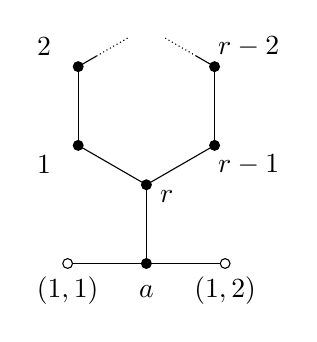
\begin{tikzpicture}[
  thin,
  vertex/.style={circle,draw=black,fill=black,inner sep=1.25pt,
    minimum size =0mm},
  attach/.style={circle,draw=black,fill=white,inner sep=1.25pt,
    minimum size =0mm},
  dots/.style={circle,fill=black,inner sep=.5pt,
    minimum size= 0pt}]
    \draw (-1,-2) -- (1,-2);
    \draw (0,-2) -- (0,-1);
    
    \node[attach] at (-1,-2) {};
    \node at (-1,-2.35) {$(1,1)$};
    \node[attach] at (1,-2) {};
    \node at (1,-2.35) {$(1,2)$};
    \node[vertex] at (0,-2) {};
    \node at (0,-2.35) {$a$};
    
    \foreach \t in {150, 210, 270, 330, 30}{
      \node[vertex] at (\t: 1) {};
    }
    
    \foreach \t in {210, 270, 330, 30}{
      \draw (\t:1) -- (\t - 60:1);
    }
    
    \draw (150:1) -- (135:.897);
    \draw (30:1) -- (45:.897);
    
    \draw[densely dotted] (45:.897) -- (75:.897);
    \draw[densely dotted] (135:.897) -- (105:.897);
    
    \foreach \t / \n in {210 / 1, 150 / 2, 30 / {r-2}, -30 / {r-1}}{
      \node at (\t:1.5) {$\n$};
    }
    
    \node at (.26,-1.15) {$r$};
  
\end{tikzpicture}
  \caption{An R/T gadget built from an $r$-cycle.}
  \label{fig:RT_cycle}
\end{figure}


To see which momenta perfectly transmit, we use \lem{transmit_reqs}. Consider the induced subgraph obtained by removing vertex $r$. This subgraph is a path of length $r-2$ and has eigenvalues $2\cos(\pi m/r)$ for $m \in [r-1]$ as discussed in the previous section. Using the expression \eq{vecs_line} for the eigenvectors, we see that the sum of the amplitudes on the two ends is nonzero for odd values of $m$.  Perfect transmission occurs for each of the corresponding momenta:  
\[
  \mathcal{T}_{\mathrm{cycle}} = \left\{ -\frac{\pi j}{r} \colon \text{$j$ is odd and $j\in [r-1]$}\right\}.
\]

For example, the $4$-cycle (i.e., square) has $\mathcal{T}_{\mathrm{cycle}} = \{-\frac{\pi}{4},-\frac{3\pi}{4}\}$ and $\mathcal{R}_{\mathrm{cycle}} = \{-\frac{\pi}{2}\}$.  


%%%%%%%%%%%%%%%%%%%%%%%%%%%%%%%%%%%%%%%%%%%%%%%%%%%%%%%%%%%%%%%%%

\subsection{Momentum switches}

\todo{Go over this section, and revise/make it fit}

To construct momentum switches between pairs of momentum, it will be worthwhile to first construct two R/T gadgets between the two momenta, with the two gadgets having swapped reflection and transmission sets.  We will then construct something like a railroad switch, by placing the two gadgets immediately after a 3-claw; this construction will then be that the wavepacket will only see one of the two outgoing paths, and function exactly how we want it to.


We now construct a momentum switch between the reflection and transmission sets $\mathcal{R}$ and $\mathcal{T}$ of a type 2 R/T gadget.  We attach the gadget and its reversal (defined in \sec{reversal}) to the leaves of a claw, as shown in \fig{gen_mom_con}.  Specifically, given a type 2 R/T gadget $\hat{G}$, the corresponding momentum switch $\hat{G}^{\prec}$ consists of a copy of $G_0$, a copy of $G_{0}^{\leftrightarrow}$, and a claw.  The three leaves of the claw are the terminals.  Vertex $p$ of $G_0$ is connected to leaf $2$ of the claw, and vertices $w_1^{(1)},\ldots,w_r^{(1)}$ of $G_{0}^{\leftrightarrow}$ are each connected to leaf $3$ of the claw.

The high-level idea of the switch construction is as follows.  For momenta in the transmission set, the gadget perfectly transmits while its reversal perfectly reflects, so the claw is effectively a path connecting terminals 1 and 2.  For momenta in the reflection set, the roles of transmission and reflection are reversed, so the claw is effectively a path connecting terminals 1 and 3.


\begin{lemma}\label{lem:mom_switch_construction}
Let $\hat{G}$ be a type 2 R/T gadget with reflection set $\mathcal{R}$ and transmission set $\mathcal{T}$.  The gadget $\hat{G}^{\prec}$ described above is a momentum switch between $\mathcal{R}$ and $\mathcal{T}$.
\end{lemma}


\begin{proof}

We construct a scattering eigenstate for each momentum $k\in \mathcal{T}$ with perfect transmission from path 1 to path 2, and similarly construct a scattering eigenstate for each momentum $k^{\prime}\in \mathcal{R}$ with perfect transmission from 1 to 3.  These eigenstates show that $S_{2,1}(k) = 1$ and $S_{3,1}(k^\prime) = 1$. Since the S-matrix is symmetric and unitary, this gives the complete form of the S-matrix for all momenta in $\mathcal{R}\cup\mathcal{T}$.  In particular, this shows that $\hat{G}^{\prec}$ is a momentum switch between $\mathcal{R}$ and $\mathcal{T}$.

We first construct the scattering states for momenta $k\in \mathcal{T}$.  \lem{transmit_reqs} shows that the graph $g_0$ has a $2\cos(k)$-eigenvector $\ket{\xi_k}$ satisfying equation \eq{trans_cond} with some nonzero constant $c$. We define a state $\ket{\mu_k}$ on $G^{\prec}$ and we show that it is a scattering eigenstate with perfect transmission between paths $1$ and $2$.   The amplitudes of $\ket{\mu_k}$ on the semi-infinite paths and the claw are
\[
  \langle (x,1)|\mu_k\rangle=e^{-ikx} \qquad 
  \langle 0|\mu_k\rangle=1 \qquad 
  \langle (x,2)|\mu_k\rangle=e^{ikx} \qquad
  \langle (x,3)|\mu_k\rangle=0.
\]
The rest of the graph consists of the three copies of the subgraph $g_0$ and the vertices $p$ and $u_{\leftrightarrow}$. The corresponding amplitudes are
\[
  \braket{v}{\mu_k} =
  \begin{cases}
	  -\frac{1}{c}\braket{v}{\xi_k} & v\in V(g^{(1)}_0) \\
    \frac{1}{c}\braket{v}{\xi_k} & v \in V(g^{(2)}_0) \\
	  -\frac{e^{ik}}{c} \braket{v}{\xi_k} & v \in V(g^{(3)}_0) \\
  	0 & v=p \text{ or } v=u_{\leftrightarrow}.
  \end{cases}
\]

We claim that $\ket{\mu_k}$ is an eigenstate of the Hamiltonian with eigenvalue $2\cos(k)$.  As in previous proofs, the state clearly satisfies the eigenvalue condition on the semi-infinite paths and at the vertices of $G_0$ and $G_0^\leftrightarrow$, and the factors of $\frac{1}{c}$ in the above equation are chosen so that it also satisfies the eigenvalue condition at vertices $p$ and $u_\leftrightarrow$. Since $\ket{\mu_k}$ is a scattering state with perfect transmission from path 1 to path 2, we see that $S_{2,1}(k) = 1$.

Finally, we construct an eigenstate $\ket{\nu_{k^\prime}}$ with perfect transmission from path 1 to path 3 for each momentum $k^\prime \in \mathcal{R}$.  This state has the form
\[
  \langle (x,1)|\nu_{k^\prime}\rangle=e^{-i k^\prime x} \qquad 
  \langle 0|\nu_{k^\prime}\rangle=1 \qquad 
  \langle (x,2)|\nu_{k^\prime}\rangle=0 \qquad
  \langle (x,3)|\nu_{k^\prime}\rangle=e^{i k^\prime x}
\]
on the semi-infinite paths and the claw.  \lem{reflect_reqs} shows that $G_0$ has a $2\cos(k^\prime)$-eigenstate $\ket{\chi_{k^\prime}}$ with $\braket{p}{\chi_{k'}} \ne 0$, which determines the form of $\ket{\nu_{k^\prime}}$ on the remaining vertices:
\[
  \braket{v}{\nu_{k^\prime}} =
  \begin{cases}
	  -\frac{1}{\braket{p}{\chi_{k'}}} \braket{v}{\chi_{k^\prime}} & v \in V(G_0) \\
	  -\frac{e^{ik'}}{\braket{p}{\chi_{k'}}} \braket{v}{\chi_{k^\prime}} & v \in V(g_0^{(2)}) \\
	  -e^{ik'} & v=u^\leftrightarrow \\
    0 & \text{otherwise}.
  \end{cases} 
\]
As before, it is easy to check that this a momentum-$k^\prime$ scattering state with perfect transmission from path 1 to path 3, so $S_{3,1}(k^\prime)=1$.

Thus the gadget from \fig{gen_mom_con} is a momentum switch between $\mathcal{R}$ and $\mathcal{T}$.
\end{proof}

\subsubsection{Explicit examples}



\todo{work this section}


%%%%%%%%%%%%%%%%%%%%%%%%%%%%%%%%%%%%%%
\subsection{Encoded unitaries}

While there is no efficient method to find graphs that apply some fixed encoded unitary, it is possible to search over all small graphs that have some particular implementation.

\missingcite{Find this small graphs thing}

Essentially, the main idea behind this method is that since we can easily compute the scattering matrix for a particular graph at a particular momentum, if we want to find a graph that has some prescribed scattering behavior at a prescribed momenta we simply assume that such a graph exists with a particular number of internal vertices, and then search over all graphs of that size.  While this exhaustive search is not guaranteed to find such a graph, a surprising number of systems can be found with this structure.  

In particular, if we restrict ourselves to simple momenta, in which the energy $2\cos(k)$ is in some simple extension of the rationals, then most simple scattering behaviors can be found.  

Graphs that end up being of particular use are those that allow for encoded unitary transformations.  As such, we want to find graphs in which the attached paths can be partitioned into two sets, corresponding to input paths and output paths.  We then want the scattering matrices at some particular momenta to be block matrices, with the diagonal blocks being zero matrices.

While this puts a large restriction on the graphs, many such graphs have been found.  In particular \missingcite{small graphs scattering stuff} has run an exhaustive search for such matrices up to size \todo{find size}.  Some graphs that will be of particular interest to us are those that serve as a universal set of gates at two particular momenta.  In particular, we will find uses for graphs that at momenta $-\frac{\pi}{4}$ implement a phase gate and implement a basis changing gate, and graphs that at momenta $-\frac{\pi}{2}$ implement a Hadamard gate. 

These graphs are as follows:
\todo{show these graphs}


%%%%%%%%%%%%%%%%%%%%%%%%%%%%%%%%%%%%%%%%%%%%%%%%%%%%%%%%%%%%%%%%%

%%%%%%%%%%%%%%%%%%%%%%%%%%%%%%%%%%%%%%%%%%%%%%%%%%%%%%%%%%%%%%%%%
\section{Various facts about scattering}

While we have the previous constructions that yield graphs with particular behavior, we will also want to understand some simple relations between graphs and their respective scattering matrices.  In particular, understanding what properties are necessary in order to have a given scattering matrix, and understanding the relation between various the scattering matrices of various momenta.

\subsection{Degree-3 graphs are sufficient}

One of the most simple assumptions that could be made is that certain scattering behaviors require high degree graphs.  In particular, the idea that having many connections might allow for some additional correlations between the outputs on larger graphs.  

If we restrict our attention to only a finite number of rational momenta, however, this does not turn out to be the case.  We can show that any graph can be replaced by a degree three graph with an identical scattering behavior at some fixed momenta.  In particular, we show that a single vertex can be replaced by a finite path while still satisfying the eigenvalue equation at some fixed momenta, which determine the length of the path.

As a degree two graphs are the graph joins of cycles and paths, degree three graphs are the smallest graphs to have nontrivial scattering behaviors.  This lemma shows that, in a certain sense, they are also all that are required.


\begin{lemma} Let $\widehat{G}$ be a finite graph, and let $M$ be a finite set of rational multiples of $\pi$.  If $v\in V(G)$ is a degree $d$ vertex, there exists a graph $H$ that extends $G$ with the vertex $v$ being replaced by a degree-$(\lceil \frac{d}{2}\rceil +1)$ subgraph such that the scattering matrices at the momenta $k\in M$ are preserved.
\label{lem:degree_reduction}
\end{lemma}
\begin{proof}
  The main idea behind this proof is to partition the vertices adjacent to $v$ into two sets, and then replace $v$ by a finite path, with the two sets connected to opposites ends of the finite path.  By choosing the length of the path correctly, we can show that the amplitudes at either end of the path can be taken as the same amplitude of $v$ at each momenta in $M$, so that the eigenvalue equation remains satisfied with the same amplitudes on every vertex other than $v$, keeping the scattering matrices the same.  
  
  In particular, let $v$ be the degree $d$ vertex in $G$, and let $S = \{w\in V(G) : w\sim v\}$.  Additionally, let us arbitrarily partition $S$ into two sets, $S_1$ and $S_2$, such that $\big||S_1|-|S_2|\big| \leq 1$.
  
  As each $k\in M$ is a finite set of rational multiples of $\pi$, there exists some $m'\in \NN$ such that for each $k\in M$, $mk = 2\pi j$ for some $j\in \NN$.  Let us then examine the graph $H$ where $v$ is replaced by a path of length $m+1$ and $S_1$ is attached to one end of the path while $S_2$ is attached to the other end.  Explicitly:
  \begin{align}
    V(H) &= V(G)\setminus \{v\} \cup \{(v,j): j\in [m+1]\}\\
    E(H) &= \big\{ e\in E(G) : v\notin e\big\} \cup \big\{ \{(v,j),(v,j+1)\} : j\in [m]\big\} \cup \nonumber\\
    &\qquad \big\{ \{s, (v,0)\} : s\in S_1\big\} \cup \big\{ \{s,(v,m)\} : s\in S_2\big\}.
  \end{align}
  
  Now, for any $k\in M$, let $\ket{\phi}$ be an eigenstate of $A(G)$ with eigenvalue $2\cos(k)$.  We will show that there exists an eigenstate $\ket{\psi}$ of $A(H)$ with energy $2\cos(k)$ such that for any $w\in V(G)\setminus \{v\}$, $\braket{w}{\phi} = \braket{w}{\psi}$.  Concretely, for any vertex other than $v$, let us define $\ket{\psi}$ in this manner, and note that $\ket{\psi}$ satisfies the eigenvalue equation with energy $2\cos(k)$ for all vertices other than those in $S$ or those replacing $v$ by assumption.  Additionally, let 
  \begin{equation}
    \alpha = \sum_{w\in S_1} \braket{w}{\phi} \qquad \beta = \braket{v}{\phi} \qquad \gamma = \sum_{w\in S_2} \braket{w}{\phi}.
  \end{equation}
  We will then defined the amplitude along the path replacing the vertex $v$ as
  \begin{equation}
    \braket{(v,j)}{\psi} = \beta \cos(k j) + \frac{\gamma - \beta\cos(k)}{\sin(k)} \sin( k j).
  \end{equation}
  Note that $\braket{(v,0)}{\psi} = \braket{(v,m)}{\psi} = \beta = \braket{v}{\phi}$, and thus the eigenvalue equation is satisfied at all vertices in $S$ with energy $2\cos(k)$.  As the eigenstates along a path with energy $2\cos(k)$ are scalar multiples of $\sin(k x)$ and $\cos(k j)$, we can also see that the eigenvalue equation is necessarily satisfied for all $(v,j)$ with $j\neq 0$ and $j\neq m$.
  
  If we then examine the eigenvalue equation at $(v,0)$, we can see that
  \begin{align}
    \sum_{s\in S_1} \braket{s}{\psi} + \braket{(v,1)}{\psi} &= \alpha + \beta \cos(k) + \frac{\gamma - \beta \cos(k)}{\sin(k)} \sin (k) \\
      &= \alpha + \gamma \\
      &= 2 \cos(k) \beta = 2 \cos(k) \braket{(v,0)}{\psi}
  \end{align}
  where the third equality follows from the fact that $\ket{\phi}$ satisfies the eigenvalue equation at $v$ with eigenvalue $2\cos(k)$. 
  
  Let us finally examine the eigenvalue equation at $(v,m)$, noting that
  \begin{align}
    \sum_{s\in S_2} \braket{s}{\psi} + \braket{(v,m-1)}{\psi} &=\gamma + \beta \cos(k (m-1)) + \frac{\gamma - \beta \cos(k)}{\sin(k)} \sin (k(m-1)) \\
      &= \gamma + \beta \cos(k)   -  \big(\gamma - \beta \cos(k)\big)\\
      &= 2 \cos(k) \beta = 2 \cos(k) \braket{(v,0)}{\psi}
  \end{align}
  where the second equality follows from some trigonometric identities. We can then see that $\ket{\psi}$ satisfies the eigenvalue equation at $(v,m)$ with energy $2\cos(k)$.
  
  Putting this together, we have that $\ket{\psi}$ is an eigenvector of $A(H)$ with energy $2\cos(k)$ such that $\ket{\psi}$ and $\ket{\phi}$ are identical on those vertices contained in both $G$ and $H$.  As this result holds for any energy $2\cos(k)$ eigenvector of $A(G)$, and as the two graphs are identical along the semi-inifinite paths, we have that the scattering matrices for these two graphs are identical, and thus the scattering matrices are preserved under this degree reduction procedure.
\end{proof}

By repeated use of this lemma, we can then see that if we are only interested in the scattering behavior of a graph at particular momenta, then we need only examine degree three graphs.


%%%%%%%%%%%%%%%%%%%%%%%%%%%%%%%%%%%%%%%%%%%%%%%%%%%%%%%%%%%%%%%%%

\subsection{Not all momenta can be split}

In addition, it might be useful to see when particular scattering behavior is possible or not.  As such ,we will show that no momentum switch can exist between the pairs of momenta $-\frac{\pi}{4}$ and $-\frac{3\pi}{4}$.  The proof will actually show that no R/T gadget exists between these two momenta, but as any momentum switch can be turned into an R/T gadget, this will be sufficient.

\todo{Go over this section, and revise}

\subsubsection{Basis vectors with entries in $\QQ(\sqrt{2})$}
\label{sec:vecs_over_field}

Recall the general setup shown in \fig{basic_scattering}: $N$ semi-infinite paths are attached to a finite graph $\hat G$. Consider an eigenvector $\ket{\tau_k}$ of the adjacency matrix of $G$ with eigenvalue $2\cos(k)$ for $k\in (-\pi,0)$. In general this eigenspace is spanned by incoming scattering states with momentum $k$ and confined bound states \cite{CG12} (which have zero amplitude on the semi-infinite paths). We can thus write the amplitudes of $\ket{\tau_k}$ on the semi-infinite paths as
\[
  \braket{(x,j)}{\tau_k} 
  = \kappa_j \cos(k (x-1)) + \sigma_j \sin(k (x-1))
\]
for $x \in \posint$, $j \in [N]$, and $\kappa_j,\sigma_j \in \CC$, and the amplitudes on the internal vertices as
\[
  \braket{w}{\tau_k} = \iota_w
\]
for $\iota_w \in \CC$, where $w$ indexes the internal vertices. We write the adjacency matrix of $\hat{G}$ as a block matrix as in \eq{blockadj}.  Since the state $\ket{\tau_k}$ satisfies the eigenvalue equation on the semi-infinite paths, it remains to satisfy the conditions specified by the block matrix equation
\begin{equation*}
  \begin{pmatrix} A & B^\dag\\ B & D\end{pmatrix}
	\begin{pmatrix} \kappa \\ \iota \end{pmatrix}
	+ \cos(k) \begin{pmatrix} \kappa \\ 0 \end{pmatrix}
	+ \sin(k) \begin{pmatrix} \sigma \\ 0 \end{pmatrix} 
	= 2\cos(k) \begin{pmatrix} \kappa \\ \iota \end{pmatrix}.
\end{equation*}

Hence, the nullspace of the matrix
\[
  M= \begin{pmatrix} A -\cos(k) \II & \sin(k) \II & B^\dag\\
    0 & 0 & 0\\
    B & 0 & D-2\cos(k)\II\end{pmatrix}
\]
is in one-to-one correspondence with the $2\cos(k)$-eigenspace of the infinite matrix (here the first block corresponds to $\kappa$, the second to $\sigma$, and the third to $\iota$). Further, $M$ only has entries in $\QQ(\cos(k),\sin(k))$, so its nullspace has a basis with amplitudes in $\QQ(\cos(k),\sin(k))$, as can be seen using Gaussian elimination.

We are interested in the specific cases $2\cos(k)=\pm\sqrt{2}$ corresponding to $k = -\frac{\pi}{4}$ or $k = -\frac{3\pi}{4}$.  In these cases $\QQ(\cos(k),\sin(k)) = \QQ(\sqrt{2})$, and we may choose a basis for the nullspace of $M$ with amplitudes from $\QQ(\sqrt{2})$. Furthermore, $\cos(kx), \sin(kx) \in \QQ(\sqrt{2})$ for all $x\in \posint$, so with such a choice of basis, each amplitude of $\ket{\tau_k}$ is also an element of $\QQ(\sqrt{2})$.

As noted above, the spectrum of $G$ may include confined bound states \cite{CG12} with eigenvalue $\pm\sqrt2$.  However, any such states are eigenstates of the adjacency matrix of $\hat{G}$ subject to the additional (rational) constraints that the amplitudes on the terminals are zero.  As such, the confined bound states have a basis over $\QQ(\sqrt{2})$. We can use this basis to restrict attention to those states orthogonal to confined bound states using only constraints over $\QQ(\sqrt{2})$, so there exists a basis over $\QQ(\sqrt{2})$ for the $N$-dimensional subspace of scattering states with energy $\pm\sqrt{2}$ that are orthogonal to the confined bound states. Finally, since $\QQ(\sqrt{2})$ can be seen as a two-dimensional vector space over $\QQ$, note that for any member of this basis $\ket{\tau_k}$ there exist rational vectors $\ket{u_k},\ket{w_k}$ such that $\ket{\tau_k}=\ket{u_k} + \sqrt{2}\ket{w_k}$. Since $H^2\ket{\tau_k}=2\ket{\tau_k}$, we have $H\ket{u_k}=\pm 2\ket{w_k}$ and $H\ket{w_k} = \pm \ket{u_k}$, so
\begin{equation}
  \ket{\tau_k}=(H \pm \sqrt{2} \II)\ket{w_k}.\label{eq:form_of_tau}
\end{equation}

%================================================================
\subsubsection{No R/T gadget and hence no momentum switch}

Recall from \sec{mswitch} that a momentum switch between two momenta $k$ and $p$ can always be converted into an R/T gadget between $k$ and $p$. Here we show that if an R/T gadget perfectly reflects at momentum $-\frac{\pi}{4}$, then it must also perfectly reflect at momentum $-\frac{3\pi}{4}$. This implies that no R/T gadget exists between these two momenta, and thus no momentum switch exists.

We use the following basic fact about two-terminal gadgets several times: 


\begin{fact}\label{fct:zero_ampl}
If a two-terminal gadget has a momentum-$k$ scattering state $\ket{\phi}$ with zero amplitude along path $2$, then the gadget perfectly reflects at momentum $k$.
\end{fact}


\begin{proof}
Without loss of generality, we may assume that $\ket{\phi}$ is orthogonal to all confined bound states.
If $\ket{\phi}$ has zero amplitude along path $2$, then there exist some $\mu,\nu \in \CC$ such that
\[
  \braket{(x,2)}{\phi}
  = \mu \braket{(x,2)}{\sc_2 (k)} + \nu \braket{(x,2)}{\sc_1(k)}
  = \mu e^{-ikx} + \mu R e^{ikx} + \nu T e^{ikx}
  = 0
\] 
for all $x\in \ZZ^{+}$.  Since this holds for all $x$, we have $\mu = \mu R + \nu T = 0$.  Since $\mu$ and $\nu$ cannot both be zero, we have $T=0$.
\end{proof}

For an R/T gadget, the scattering states (at some fixed momentum) that are orthogonal to the confined bound states span a two-dimensional space. As shown in \sec{vecs_over_field}, we can expand each scattering eigenstate at momentum $k=-\frac{\pi}{4}$ in a basis with entries in $\QQ(\sqrt{2})$, where each basis vector takes the form \eq{form_of_tau}. This gives
\begin{equation*}
  \ket{\sc_{1}(-\tfrac{\pi}{4})} 
  = (H + \sqrt{2}\II) (\alpha \ket{a} + \beta \ket{b}) \label{eq:rat_expansion}
\end{equation*}
where $\alpha,\beta \in \CC$, $\alpha\neq 0$, and $\ket{a}$ and $\ket{b}$ are rational 2-eigenvectors of $H^2$.

If $T(-\frac{\pi}{4}) = 0$, then for all $x \geq 0$, 
\[
  \langle x,2\ket{\sc_1(-\tfrac{\pi}{4})} 
  = 0 
  = \langle{x,2} |(H + \sqrt{2}\II) (\alpha \ket{a} + \beta \ket{b}).
\]
Dividing through by $\alpha$ and rearranging, we get that for all $x\geq 0$,
\begin{equation*}
\frac{\beta}{\alpha} (\langle{x,2}| H\ket{b}+\sqrt{2} \langle{x,2}\ket{b})
  =-\langle{x,2}| H\ket{a}  -\sqrt{2} \langle{x,2}\ket{a}.
\label{eq:cases_eqn}
\end{equation*}
If the left-hand side is not zero, then $\beta/\alpha \in \QQ(\sqrt{2})$ since $H$, $\ket{a}$, and $\ket{b}$ are rational.  If the left-hand side is zero, then $(H+ \sqrt{2}\II)\ket{a}$ is an eigenstate at energy $2\cos(k)$ with no amplitude along path 2, so $\beta = 0$ (using \fct{zero_ampl}), and again $\beta/\alpha \in \QQ(\sqrt{2})$.

Now write $\beta/\alpha=r+s\sqrt{2}$ with $r,s\in\QQ$, and consider the rational 2-eigenvector of $H^2$
\[
  \ket{c} := \ket{a} + (r+sH) \ket{b}.
\]
Note that
\[
  \alpha (H + \sqrt{2} \II) \ket{c} 
= \alpha(H+ \sqrt{2} \II) \ket{a} + \alpha (rH+r\sqrt{2}+ sH^2+sH\sqrt{2}) \ket{b}.
\]
Since $\ket{b}$ is a 2-eigenvector of $H^2$ and $\beta/\alpha=r+s\sqrt{2}$, this simplifies to
\begin{equation}
  \alpha (H + \sqrt{2}\II) \ket{c} 
  = \alpha (H + \sqrt{2}\II) \ket{a} + \beta(H + \sqrt{2}\II) \ket{b} 
  = \ket{\sc_1(-\tfrac{\pi}{4})}, \label{eq:sc1_c}
\end{equation}
so $\ket{\sc_1(-\tfrac{\pi}{4})}$ can be written as $\alpha(H+\sqrt{2}\II)$ times a rational 2-eigenvector of $H^2$.

Since $\langle{x,2}\ket{\sc_1(-\tfrac{\pi}{4})} = 0$ for all $x\geq 1$ (and $\alpha\neq 0$), we have
\[
  \langle{x,2}| (H+\sqrt{2}\II) \ket{c} 
  = \langle{x,2}| H \ket{c} + \sqrt{2} \langle{x,2}\ket{c} 
  = 0.
\]
As $H$ is a rational matrix and $\ket{c}$ is a rational vector, the rational and irrational components must both be zero, implying $\langle{x,2}\ket{c}  =\langle{x,2}|H\ket{c} = 0$ for all $x\geq 1$. Furthermore, since $ \ket{\sc_1(-\tfrac{\pi}{4})}$ is a scattering state with zero amplitude on path $2$, it must have some nonzero amplitude on path 1 and thus there is some $x_0\in \mathbb{Z}^+$ for which $\langle{x_0,1}\ket{c}\neq 0$ or $\langle{x_0,1}|H\ket{c} \neq 0$.

Now consider the state obtained by replacing $\sqrt{2}$ with $-\sqrt{2}$:
\[
  \ket{\overline{\sc}_1(-\tfrac{\pi}{4})} := \alpha (H-\sqrt{2}\II) \ket{c}.
\]
This is a $-\sqrt{2}$-eigenvector of $H$, which can be confirmed using the fact that $\ket{c}$ is a $2$-eigenvector of $H^2$. As $\langle{x,2} | H \ket{c} = \langle x,2 \ket{c} = 0$ for all $x\geq 1$, $\langle x,2 \ket{\overline{\sc}_1(-\tfrac{\pi}{4})} = 0$ for all $x\geq 1$. Furthermore the amplitude at vertex $(x_0,1)$ is nonzero, i.e.,  $\langle x_0,1 \ket{\overline{\sc}_1(-\tfrac{\pi}{4})} \neq 0$, and hence $\ket{\overline{\sc}_1(-\tfrac{\pi}{4})}$ has a component orthogonal to the space of confined bound states (which have zero amplitude on both semi-infinite paths).  Hence, there exists a scattering state with eigenvalue $-\sqrt{2}$ with no amplitude on path 2. By \fct{zero_ampl}, the gadget perfectly reflects at momentum $-\frac{3\pi}{4}$.  It follows that no perfect R/T gadget (and hence no perfect momentum switch) exists between these momenta.

This proof technique can also establish non-existence of momentum switches between other pairs of momenta $k$ and $p$.  For example, a slight modification of the above proof shows that no momentum switch exists between $k = -\frac{\pi}{6}$ and $p = -\frac{5\pi}{6}$. 

%%%%%%%%%%%%%%%%%%%
\subsection{Laplacians vs adjacency matrix}

\todo{If I have time, write this section}

%%%%%%%%%%%%%%%%%%%%%%%%%%%%%%%%%%%%%%%%%%%%%%%%%%%%%%%%%%%%%%%
\section{Finite truncation}

\section{Finite truncation}

While the intuition all deals with infinite paths and wavepackets with some exact momenta, we will unfortunately have to deal with finite approximations to these ideals.  While the \lem{truncation_lemma} deals with the finite sized graphs, the restriction to finite sized wavepackets will unfortunately be slightly more complicated.

Unfortunately, much of this complication arises from the simple fact that the time evolved wavepackets do not have a nice form, and thus our approximations to these wavepackets are somewhat cumbersome.  However, if we assume that the initial wavepacket was a a square window on the momenta of interest some distance from the finite sized graph, the time evolved state essentially has the same state moved forward in time.


%%%%%%%%%%%%%%%%
% Wavepacket scattering

\begin{theorem} Let $\widehat{G}$ be an $(N+m)$-vertex graph.  Let $G$ be the graph obtained from $\widetilde{G}$ by attaching semi-infinite paths to the first $N$ of its vertices, and let $S$ be the corresponding $S$-matrix.  Let $H_G$ be the quantum walk Hamiltonian of equation \missingcite{correct equation}. Let $k\in (-\pi,0)$, $M,L\in \NN$, $j\in [N]$, and 
\begin{equation}
  \ket{\psi^j(0)} = \frac{1}{\sqrt{L}} \sum_{x=M+1}^{M4L} e^{-i k x} \ket{x,j}.
\end{equation}
Let $c_0$ be a constant independent of $L$.  Then, for all $0 \leq t \leq c_0 L$,
\begin{equation}
   \Big\|e^{-i H_G t}\ket{\psi^j(0)} - \ket{\alpha^j(t)}\Big\| = \OO(L^{-1/4})
\end{equation}
where
\begin{equation}
  \ket{\alpha^j(t)} = \frac{1}{\sqrt{L}} e^{-2 i t \cos k} \sum_{x=1}^\infty \sum_{q=1}^N (\delta_{qj} e^{-ikx} R(x- \lfloor 2t \sin k\rfloor ) + S_{qj}(k) e^{ikx} R(-x - \lfloor 2t \sin k\rfloor ) ) \ket{x,q}
\end{equation}
with
\begin{equation}
  R(l) = \begin{cases} 1 & \text{ if } l- M \in [L]\\
    0 & \text{ otherwise.}
    \end{cases}
\end{equation}
\label{thm:SP_wavepacket}
\end{theorem}
n this section we prove \thm{singlepart}. The proof is based on (and follows closely) the calculation from the appendix of reference \cite{FGG08}.

Recall from \eq{single_particle_states} that the scattering eigenstates of $H_{G}^{(1)}$ have the
form
\[
\langle x,q|\text{sc}_{j}(k)\rangle=e^{-ikx}\delta_{qj}+e^{ikx}S_{qj}(k)\]
 for each $k\in(-\pi,0)$. 

Before delving into the proof, we first establish that the state $|\alpha^{j}(t)\rangle$ is approximately normalized. This state is not normalized at all times $t$. However, $\langle\alpha^{j}(t)|\alpha^{j}(t)\rangle=1+\OO(L^{-1})$, as we now show:
\begin{align*}
\langle\alpha^{j}(t)|\alpha^{j}(t)\rangle & =\frac{1}{L} \sum_{x=1}^{\infty}\left|e^{-ikx}R(x-\left\lfloor 2t\sin k\right\rfloor)+S_{jj}(k)e^{ikx}R(-x-\left\lfloor 2t\sin k\right\rfloor)\right|^{2} \\
 &\quad   +\frac{1}{L}\sum_{q\neq j}\sum_{x=1}^{\infty}|S_{qj}(k)|^{2} R(-x-\left\lfloor 2t\sin k\right\rfloor) \\
 & = \frac{1}{L}\sum_{x=1}^{\infty}\left[R(x-\left\lfloor 2t\sin k\right\rfloor )+R(-x-\left\lfloor 2t\sin k\right\rfloor)\right] \\
 &  \quad +\frac{1}{L}\sum_{x=1}^{\infty}\left(e^{-2ikx}S_{jj}^{\ast}(k)+e^{2ikx}S_{jj}(k)\right)R(x-\left\lfloor 2t\sin k\right\rfloor)R(-x-\left\lfloor 2t\sin k\right\rfloor) \\
 & = 1\! +\! \frac{1}{L}\sum_{x=1}^{\infty}
 	\left(e^{-2ikx}S_{jj}^{\ast}(k)\! +\! e^{2ikx}S_{jj}(k)\right)
   R(x\! -\! \left\lfloor 2t\sin k\right\rfloor)
   R(-x\! -\!\left\lfloor 2t\sin k\right\rfloor)
   \! +\!\OO(L^{-1})
\end{align*}
where we have used unitarity of $S$ in the second step.
When it is nonzero, the second term can be written as
\[
\frac{1}{L}\sum_{x=1}^{b}\left(e^{-2ikx}S_{jj}^{\ast}(k)+e^{2ikx}S_{jj}(k)\right)
\]
where $b$ is the maximum positive integer such that $\{-b,b\}\subset\{M+1+\left\lfloor 2t\sin k\right\rfloor,\ldots,M+L+\left\lfloor 2t\sin k\right\rfloor \}$. Performing
the sums, we get
\begin{align*}
\left|\frac{1}{L}\sum_{x=1}^{b}\left(e^{-2ikx}S_{jj}^{\ast}(k)+e^{2ikx}S_{jj}(k)\right)\right| 
&= \frac{1}{L} \left|S_{jj}^{\ast}(k)e^{-2ik} \frac{e^{-2ikb}-1}{e^{-2ik}-1} 
+
S_{jj}(k)e^{2ik} \frac{e^{2ikb}-1}{e^{2ik}-1} \right|\\
 & \leq \frac{2}{L|{\sin k}|} .
\end{align*}

Thus we have $\langle\alpha^{j}(t)|\alpha^{j}(t)\rangle=1+\OO(L^{-1})$.

\begin{proof}[Proof of {\thm{singlepart}}]
Define
\[
|\psi^{j}(t)\rangle=e^{-iH_{G}^{(1)}t}|\psi^{j}(0)\rangle
\]
and write
\[
|\psi^{j}(t)\rangle=|w^{j}(t)\rangle+|v^{j}(t)\rangle
\]
where
\[
|w^{j}(t)\rangle=\int_{-\epsilon}^{\epsilon}\frac{d\phi}{2\pi}e^{-2it\cos\left(k+\phi\right)}\sum_{q=1}^{N}|\text{sc}_{q}(k+\phi)\rangle\langle\text{sc}_{q}(k+\phi)|\psi^{j}(0)\rangle
\]
and $\langle w^{j}(t)|v^{j}(t)\rangle=0$. We take $\epsilon=\frac{\left|\sin k\right|}{2\sqrt{L}}$.
Now \[
\langle\text{sc}_{q}(k+\phi)|\psi^{j}(0)\rangle=\frac{1}{\sqrt{L}}\sum_{x=M+1}^{M+L}\left(e^{i\phi x}\delta_{qj}+e^{-i\left(2k+\phi\right)x}S_{qj}^{\ast}(k+\phi)\right),\]
 so \[
|w^{j}(t)\rangle=|w_{A}^{j}(t)\rangle+\sum_{q=1}^{N}|w_{B}^{q,j}(t)\rangle\]
 where \begin{align*}
|w_{A}^{j}(t)\rangle & = \int_{-\epsilon}^{\epsilon}\frac{d\phi}{2\pi}e^{-2it\cos\left(k+\phi\right)}f(\phi)|\text{sc}_{j}(k+\phi)\rangle\\
|w_{B}^{q,j}(t)\rangle & = \int_{-\epsilon}^{\epsilon}\frac{d\phi}{2\pi}e^{-2it\cos\left(k+\phi\right)}g_{qj}(\phi)|\text{sc}_{q}(k+\phi)\rangle
\end{align*}
with
\begin{align*}
f(\phi) & = \frac{1}{\sqrt{L}}\sum_{x=M+1}^{M+L}e^{i\phi x}\\
g_{qj}(\phi) & = \frac{1}{\sqrt{L}}\sum_{x=M+1}^{M+L}e^{-i\left(2k+\phi\right)x}S_{qj}^{\ast}(k+\phi).\end{align*}
We will see that $\ket{\psi^j(t)} \approx \ket{w^j(t)} \approx \ket{w^j_A(t)} \approx \ket{\alpha^j(t)}$.

Now
\begin{align*}
\langle w_{A}^{j}(t)|w_{A}^{j}(t)\rangle & = \int_{-\epsilon}^{\epsilon}\frac{d\phi}{2\pi}\left|f(\phi)\right|^{2}
 = \frac{1}{L} \int_{-\epsilon}^{\epsilon}\frac{d\phi}{2\pi}\frac{\sin^{2}(\frac{1}{2}L\phi)}{\sin^{2}(\frac{1}{2}\phi)}
 \end{align*}
but
\[
\frac{1}{L} \int_{-\pi}^{\pi}\frac{d\phi}{2\pi}\frac{\sin^{2}(\frac{1}{2}L\phi)}{\sin^{2}(\frac{1}{2}\phi)}=1
\]
and
\begin{align}
\frac{1}{L}\left(\int_{\epsilon}^{\pi}+\int_{-\pi}^{-\epsilon}\right)\frac{d\phi}{2\pi}\frac{\sin^{2}(\frac{1}{2}L\phi)}{\sin^{2}(\frac{1}{2}\phi)} & = \frac{2}{L} \int_{\epsilon}^{\pi}\frac{d\phi}{2\pi}\frac{\sin^{2}(\frac{1}{2}L\phi)}{\sin^{2}(\frac{1}{2}\phi)}\nonumber \\
 & \leq \frac{2}{L}\int_{\epsilon}^{\pi}\frac{d\phi}{2\pi}\frac{\pi^{2}}{\phi^{2}}\nonumber \\
 & \leq \frac{\pi}{L\epsilon}.\label{eq:fbound}
\end{align}
Therefore
\[
1\geq\langle w_{A}^{j}(t)|w_{A}^{j}(t)\rangle\geq1-\frac{\pi}{L\epsilon}.
\]
Similarly,
\[
\langle w_{B}^{qj}(t)|w_{B}^{qj}(t)\rangle=\int_{-\epsilon}^{\epsilon}\frac{d\phi}{2\pi}\frac{\left|S_{qj}(k+\phi)\right|^{2}}{L}\frac{\sin^{2}(\frac{1}{2}L(2k+\phi))}{\sin^{2}(\frac{1}{2}(2k+\phi))},\]
and, using the unitarity of $S$,
\begin{align*}
\sum_{q=1}^{N}\langle w_{B}^{qj}(t)|w_{B}^{qj}(t)\rangle & = \frac{1}{L}\int_{-\epsilon}^{\epsilon}\frac{d\phi}{2\pi}\frac{\sin^{2}(\frac{1}{2}L(2k+\phi))}{\sin^{2}(\frac{1}{2}(2k+\phi))}\\
 & \leq \frac{1}{L} \int_{-\epsilon}^{\epsilon}\frac{d\phi}{2\pi}\frac{1}{\sin^{2}(\frac{1}{2}(2k+\phi))}.
\end{align*}
Now $|{\sin(k+{\phi}/{2}) - \sin k}| \leq {|\phi|}/{2}$ (by the mean value theorem). So
\begin{align*}
\sin^{2}\left(k+\frac{\phi}{2}\right) & \geq \left(\left|\sin k\right|-\left|\frac{\phi}{2}\right|\right)^{2}.
\end{align*}
Since $\epsilon=\frac{\left|\sin k\right|}{2\sqrt{L}}<\left|\sin k\right|$
we then have \begin{align*}
\sum_{q=1}^{N}\langle w_{B}^{qj}(t)|w_{B}^{qj}(t)\rangle & \leq \frac{1}{L} \int_{-\epsilon}^{\epsilon}\frac{d\phi}{2\pi}\frac{4}{\sin^{2}k}\\
 & = \frac{4\epsilon}{\pi L\sin^{2}k}.\end{align*}
 Hence \begin{align*}
\langle w^{j}(t)|w^{j}(t)\rangle & \geq \langle w_{A}^{j}(t)|w_{A}^{j}(t)\rangle-2\left|\sum_{q=1}^{N}\langle w_{A}^{j}(t)|w_{B}^{qj}(t)\rangle\right|\\
 & \geq 1-\frac{\pi}{L\epsilon}-2\left\Vert \sum_{q=1}^{n}|w_{B}^{qj}(t)\rangle\right\Vert \\
 & \geq 1-\frac{\pi}{L\epsilon}-2\sum_{q=1}^{n}\left\Vert |w_{B}^{qj}(t)\rangle\right\Vert \\
 & \geq 1-\frac{\pi}{L\epsilon}-4\sqrt{\frac{\epsilon N}{\pi L\sin^{2}k}},\end{align*}
so
\[
\langle v^{j}(t)|v^{j}(t)\rangle\leq\frac{\pi}{L\epsilon}+4\sqrt{\frac{\epsilon N}{\pi L\sin^{2}k}}
\]
since $\langle v^{j}(t)|v^{j}(t)\rangle+\langle w^{j}(t)|w^{j}(t)\rangle=1$.
Thus
\begin{align*}
\left\Vert |\psi^{j}(t)\rangle-|w_{A}^{j}(t)\rangle\right\Vert  & = \left\Vert |v^{j}(t)\rangle+\sum_{q=1}^{N}|w_{B}^{qj}(t)\rangle\right\Vert \\
 & \leq \left(\frac{\pi}{L\epsilon}+4\sqrt{\frac{\epsilon N}{\pi L\sin^{2}k}}\right)^{\frac{1}{2}}+2\sqrt{\frac{\epsilon N}{\pi L\sin^{2}k}}.
\end{align*}
With our choice $\epsilon=\frac{\left|\sin k\right|}{2\sqrt{L}}$,
we have $\norm{|\psi^{j}(t)\rangle-|w_{A}^{j}(t)\rangle} =\O(L^{-{1}/
{4}})$.

We now show that
\begin{equation}
\left\Vert |w_{A}^{j}(t)\rangle-|\alpha^{j}(t)\rangle\right\Vert =\O(L^{-{1}/{8}}).\label{eq:alpha_w_bound}\end{equation}
Letting \[
P=\sum_{q=1}^{N}\sum_{x=1}^{\infty}|x,q\rangle\langle x,q|\]
be the projector onto the semi-infinite paths, to show equation \eq{alpha_w_bound}
it is sufficient to show that
\begin{equation}
\left\Vert P|w_{A}^{j}(t)\rangle-|\alpha^{j}(t)\rangle\right\Vert = \O(L^{-{1}/{4}})
\label{eq:bound_inside_lines}
\end{equation}
since this implies that
\begin{align*}
\left\Vert P|w_{A}^{j}(t)\rangle\right\Vert  & = \left\Vert |\alpha^{j}(t)\rangle\right\Vert + \O(L^{-{1}/{4}})\\
 & = 1+\O(L^{-{1}/{4}})
\end{align*}
and hence
\begin{align}
\left\Vert \left(1-P\right)|w_{A}^{j}(t)\rangle\right\Vert ^{2} & = \left\Vert |w_{A}^{j}(t)\rangle\right\Vert ^{2}-\left\Vert P|w_{A}^{j}(t)\rangle\right\Vert ^{2}\nonumber \\
 & \leq 1-\left(1+\O(L^{-{1}/{4}})\right)\nonumber \\
 & = \O(L^{-{1}/{4}}).\label{eq:bound_outside_lines}
\end{align}
From the above formula we now see that inequality \eq{bound_inside_lines}
implies \eq{alpha_w_bound}.

Noting that
\[
\frac{1}{\sqrt{L}}R(l)=\int_{-\pi}^{\pi}\frac{d\phi}{2\pi}e^{-i\phi l}f(\phi),
\]
we write
\begin{align}
\langle x,q|\alpha^{j}(t)\rangle & = e^{-2it\cos k}\left(\delta_{qj}e^{-ikx}\int_{-\pi}^{\pi}\frac{d\phi}{2\pi}e^{-i\phi\left(x-\left\lfloor 2t\sin k\right\rfloor \right)}f(\phi)\right.\nonumber\\
&\qquad\qquad\qquad  \left. +S_{qj}(k)e^{ikx}\int_{-\pi}^{\pi}\frac{d\phi}{2\pi}e^{-i\phi\left(-x-\left\lfloor 2t\sin k\right\rfloor \right)}f(\phi)\right).\label{eq:alpha_mat_elements}
\end{align}
On the other hand,
\begin{equation}
\langle x,q|w_{A}^{j}(t)\rangle=\int_{-\epsilon}^{\epsilon}\frac{d\phi}{2\pi}e^{-2it\cos\left(k+\phi\right)}f(\phi)\left(e^{-i\left(k+\phi\right)x}\delta_{qj}+e^{i\left(k+\phi\right)x}S_{qj}(k+\phi)\right).\label{eq:w_a_mat_elements}
\end{equation}
Using equations \eq{alpha_mat_elements} and \eq{w_a_mat_elements}
we can write\[
P|w_{A}^{j}(t)\rangle=|\alpha^{j}(t)\rangle+\sum_{i=1}^{7}|c_{i}^{j}(t)\rangle\]
 where $P|c_{i}^{j}(t)\rangle=|c_{i}^{j}(t)\rangle$ and \begin{align*}
\langle x,q|c_{1}^{j}(t)\rangle & = \delta_{qj}e^{-2it\cos k}e^{-ikx}\int_{-\pi}^{\pi}\frac{d\phi}{2\pi}e^{-i\phi x}f(\phi)\left(e^{2it\phi\sin k}-e^{i\phi\left\lfloor 2t\sin k\right\rfloor }\right)\\
\langle x,q|c_{2}^{j}(t)\rangle & = S_{qj}(k)e^{-2it\cos k}e^{ikx}\int_{-\pi}^{\pi}\frac{d\phi}{2\pi}e^{i\phi x}f(\phi)\left(e^{2it\phi\sin k}-e^{i\phi\left\lfloor 2t\sin k\right\rfloor }\right)\\
\langle x,q|c_{3}^{j}(t)\rangle & = -\delta_{qj}e^{-2it\cos k}e^{-ikx}\left(\int_{\epsilon}^{\pi}+\int_{-\pi}^{-\epsilon}\right)\frac{d\phi}{2\pi}e^{-i\phi x}f(\phi)e^{2it\phi\sin k}\\
\langle x,q|c_{4}^{j}(t)\rangle & = -S_{qj}(k)e^{-2it\cos k}e^{ikx}\left(\int_{\epsilon}^{\pi}+\int_{-\pi}^{-\epsilon}\right)\frac{d\phi}{2\pi}e^{i\phi x}f(\phi)e^{2it\phi\sin k}\\
\langle x,q|c_{5}^{j}(t)\rangle & = \delta_{qj}e^{-ikx}\int_{-\epsilon}^{\epsilon}\frac{d\phi}{2\pi}e^{-i\phi x}f(\phi)\left(e^{-2it\cos\left(k+\phi\right)}-e^{-2it\cos k+2it\phi\sin k}\right)\\
\langle x,q|c_{6}^{j}(t)\rangle & = S_{qj}(k)e^{ikx}\int_{-\epsilon}^{\epsilon}\frac{d\phi}{2\pi}e^{i\phi x}f(\phi)\left(e^{-2it\cos\left(k+\phi\right)}-e^{-2it\cos k+2it\phi\sin k}\right)\\
\langle x,q|c_{7}^{j}(t)\rangle & = e^{ikx}\int_{-\epsilon}^{\epsilon}\frac{d\phi}{2\pi}e^{i\phi x}e^{-2it\cos\left(k+\phi\right)}f(\phi)\left(S_{qj}(k+\phi)-S_{qj}(k)\right).
\end{align*}
We now bound the norm of each of these states:
\begin{align*}
\langle c_{1}^{j}(t)|c_{1}^{j}(t)\rangle & = \sum_{q=1}^{N}\sum_{x=1}^{\infty}\left|\delta_{qj}e^{-2it\cos k}e^{-ikx}\int_{-\pi}^{\pi}\frac{d\phi}{2\pi}e^{-i\phi x}f(\phi)\left(e^{2it\phi\sin k}-e^{i\phi\left\lfloor 2t\sin k\right\rfloor }\right)\right|^{2}\\
 & \leq \sum_{q=1}^{N}\sum_{x=-\infty}^{\infty}\left|\delta_{qj}e^{-2it\cos k}e^{-ikx}\int_{-\pi}^{\pi}\frac{d\phi}{2\pi}e^{-i\phi x}f(\phi)\left(e^{2it\phi\sin k}-e^{i\phi\left\lfloor 2t\sin k\right\rfloor }\right)\right|^{2}\\
 & = \int_{-\pi}^{\pi}\frac{d\phi}{2\pi}\left|f(\phi)\right|^{2}\left|e^{2it\phi\sin k}-e^{i\phi\left\lfloor 2t\sin k\right\rfloor }\right|^{2}\\
 & \leq \int_{-\pi}^{\pi}\frac{d\phi}{2\pi}\left|f(\phi)\right|^{2}\left(2t\phi\sin k-\left\lfloor 2t\sin k\right\rfloor \phi\right)^{2}\\
 & \leq \int_{-\pi}^{\pi}\frac{d\phi}{2\pi}\left|f(\phi)\right|^{2}\phi^{2}
\end{align*}
where we have used the facts that $|{e^{is}-1}|^{2} \leq s^{2}$
for $s\in\mathbb{R}$ and $\left|2t\sin k -\left\lfloor 2t\sin k\right\rfloor \right|<1$. In the above we performed the sum over $x$ using the identity
\[
\sum_{x=-\infty}^{\infty} e^{i(\phi-\tilde{\phi})x}=2\pi\delta(\phi-\tilde{\phi}) \text{ for } \phi,\tilde{\phi}\in (-\pi,\pi).
\]
We use this fact repeatedly in the following calculations.
Continuing, we get
\begin{align*}
\langle c_{1}^{j}(t)|c_{1}^{j}(t)\rangle & \leq \frac{1}{L} \int_{-\pi}^{\pi}\frac{d\phi}{2\pi}\frac{\sin^{2}(\frac{1}{2}L\phi)}{\sin^{2}(\frac{1}{2}\phi)}\phi^{2}\\
 & \le \frac{1}{L} \int_{-\pi}^{\pi}\frac{d\phi}{2\pi}\frac{1}{\sin^{2}(\frac{1}{2}\phi)}\phi^{2}\\
 & \leq \frac{\pi^{2}}{L}
\end{align*}
using the fact that $\sin^{2}({\phi}/{2})\geq{\phi^{2}}/{\pi^{2}}$
for $\phi\in[-\pi,\pi]$. Similarly we bound $\langle c_{2}^{j}(t)|c_{2}^{j}(t)\rangle\leq{\pi^{2}}/{L}$. 

Using equation \eq{fbound} we get 
\begin{align*}
\langle c_{3}^{j}(t)|c_{3}^{j}(t)\rangle & \leq \left(\int_{\epsilon}^{\pi}+\int_{-\pi}^{-\epsilon}\right)\frac{d\phi}{2\pi}\left|f(\phi)\right|^{2}\\
 & \leq \frac{\pi}{L\epsilon}\end{align*}
and similarly for $\langle c_{4}^{j}(t)|c_{4}^{j}(t)\rangle$.
Next, we have
\begin{align*}
\langle c_{5}^{j}(t)|c_{5}^{j}(t)\rangle & \leq \int_{-\epsilon}^{\epsilon}\frac{d\phi}{2\pi}\left|f(\phi)\right|^{2}\left|e^{-2it\cos\left(k+\phi\right)}-e^{-2it\cos k+2it\phi\sin k}\right|^{2}\\
 & \leq \int_{-\epsilon}^{\epsilon}\frac{d\phi}{2\pi}\left|f(\phi)\right|^{2}\left(2t\cos\left(k+\phi\right)-2t\cos k+2t\phi\sin k\right)^{2}\\
 & = \int_{-\epsilon}^{\epsilon}\frac{d\phi}{2\pi}\left|f(\phi)\right|^{2}\left(2t\cos k\left(\cos\phi-1\right)+2t\sin k\left(\phi-\sin\phi\right)\right)^{2}\\
 & \leq \int_{-\epsilon}^{\epsilon}\frac{d\phi}{2\pi}\left|f(\phi)\right|^{2}4t^{2}\phi^{4}\\
 & = \frac{4t^{2}}{L}\int_{-\epsilon}^{\epsilon}\frac{d\phi}{2\pi}\frac{\sin^{2}(\frac{1}{2}L\phi)}{\sin^{2}(\frac{1}{2}\phi)}\phi^{4}\\
 & \leq \frac{4t^{2}}{L}\int_{-\epsilon}^{\epsilon}\frac{d\phi}{2\pi}\pi^{2}\phi^{2}\\
 & = \frac{4\pi}{3L}t^{2}\epsilon^{3}\end{align*}
 and we have the same bound for $|c_{6}^{j}(t)\rangle$. Finally, 
\begin{align*}
\langle c_{7}^{j}(t)|c_{7}^{j}(t)\rangle & \leq \int_{-\epsilon}^{\epsilon}\frac{d\phi}{2\pi}\left|f(\phi)\right|^{2}\sum_{q=1}^{N}\left|S_{qj}(k+\phi)-S_{qj}(k)\right|^{2}.\end{align*}
Now, for each $q\in\{1,\ldots,N\}$,
\[
\left|S_{qj}(k+\phi)-S_{qj}(k)\right| \leq \Gamma |\phi|
\]
where the Lipschitz constant
\[
\Gamma = \max_{q,j\in\{1,\ldots,N\}} \max_{k' \in [-\pi,\pi]}\left|\frac{d}{dk'}S_{qj}(k')\right|
\]
is well defined since each matrix element $S_{qj}(k')$ is a
bounded rational function of $e^{ik'}$, as can be seen from equation \eq{smatrixgamma}. Hence
\begin{align*}
\langle c_{7}^{j}(t)|c_{7}^{j}(t)\rangle & \leq \int_{-\epsilon}^{\epsilon}\frac{d\phi}{2\pi}\left|f(\phi)\right|^{2}N\Gamma^{2}\phi^{2}\\
 & = \frac{N\Gamma^{2}}{L}\int_{-\epsilon}^{\epsilon}\frac{d\phi}{2\pi}\frac{\sin^{2}(\frac{1}{2}L\phi)}{\sin^{2}(\frac{1}{2}\phi)}\phi^{2}\\
 & \leq \frac{N\Gamma^{2}}{L}\int_{-\epsilon}^{\epsilon}\frac{d\phi}{2\pi}\pi^{2}\\
 & = N\Gamma^{2}\frac{\pi\epsilon}{L}.
\end{align*}
Now using the bounds on the norms of each of these states we get
\begin{align*}
\left\Vert P|w_{A}^{j}(t)\rangle-|\alpha^{j}(t)\rangle\right\Vert  & \leq 2\frac{\pi}{\sqrt{L}}+2\sqrt{\frac{\pi}{L\epsilon}}+2\sqrt{\frac{4\pi}{3L}t^{2}\epsilon^{3}}+\sqrt{N\Gamma^{2}\frac{\pi\epsilon}{L}}\\
 & = \O(L^{-{1}/{4}})
\end{align*}
using the choice $\epsilon=\frac{|{\sin p}|}{2\sqrt{L}}$ and the fact that $t = \O(L)$. 
\end{proof}

Note that this analysis assumes that $N = \O(1)$, which is the case in our applications of \thm{singlepart}.



%%%%%%%%%%%%%%%%%%%%%%%%%%%%%%%%%%%%%%%%%%%%%%%%%%%%%%%%%%%%%%%
\section{Conclusions and open problems}

I need to say something here.

Find more gates.

Determine necessary conditions for momentum switches to occur.

Basically just do more research.

\biblio{}

\end{document}